\documentclass[11pt,
a4paper,
numbers=nonperiod,
footsepline,
oneside,
numbers=noenddot,
bibliography=totoc
]{scrartcl}
\usepackage{scrlayer-scrpage}
\usepackage{caption}
\usepackage[pdfborder={0 0 0}]{hyperref}
\usepackage{graphicx}
\usepackage[ngerman]{babel}
\usepackage{listings}
\usepackage[utf8]{inputenc}
\usepackage{csquotes}
\usepackage[T1]{fontenc}
\usepackage{hyperref}
\usepackage{graphicx}
\usepackage{url}
\usepackage{booktabs}
\usepackage{xcolor}
\usepackage{pgfgantt}
\usepackage[left=2cm, right=2cm, top=1.50cm, bottom=2.60cm]{geometry}
\addtokomafont{sectioning}{\sffamily}
\clubpenalty = 10000
\widowpenalty = 10000
\usepackage{etoolbox}
\makeatletter
\patchcmd{\@maybeautodot}{.}{}{}{}
\makeatother
\usepackage[ngerman]{varioref} % Muss vor hyperref/cleveref geladen werden
\usepackage[ngerman]{cleveref}
\usepackage{pdfpages}

% Literaturverzeichnis-Paket laden
\usepackage[
backend=biber,      % Empfohlener Prozessor
style=numeric,      % Nummerierung [1], [2]
sorting=none,       % Erscheinen in der Reihenfolge der Nennung im Text
autocite=plain
]{biblatex}

% Die Datenbank-Datei einbinden
\addbibresource{include/quellen.bib}

% Verhindert, dass URLs über den Rand ragen
\usepackage{xurl} 
\hypersetup{breaklinks=true}
\usepackage{etoc}
\usepackage{float}

%Fusszeilen Einstellungen
\newcommand{\fusszeilentitel}{Ingo Weber} % Hier kommt Ihr Name rein
\clearpairofpagestyles
\refoot{\raisebox{-1mm}{Seite \pagemark}}
\lefoot{\raisebox{-1mm}{\fusszeilentitel}}

\rofoot{\raisebox{-1mm}{Seite \pagemark}}
\lofoot{\raisebox{-1mm}{\fusszeilentitel}}
\setcounter{secnumdepth}{3}
\setcounter{tocdepth}{3}

\definecolor{codegreen}{rgb}{0,0.6,0}
\definecolor{codegray}{rgb}{0.5,0.5,0.5}
\definecolor{codepurple}{rgb}{0.58,0,0.82}
\definecolor{backcolour}{rgb}{0.95,0.95,0.92}

% Globaler Stil für alle Listings
\lstset{
	backgroundcolor=\color{backcolour},   
	commentstyle=\color{codegreen},
	keywordstyle=\color{magenta},
	numberstyle=\tiny\color{codegray},
	stringstyle=\color{codepurple},
	basicstyle=\ttfamily\footnotesize,
	breakatwhitespace=false,         
	breaklines=true,                 % Zeilenumbruch bei zu langen Zeilen
	captionpos=b,                    
	keepspaces=true,                 
	numbers=left,                    % Zeilennummern links
	numbersep=5pt,                  
	showspaces=false,                
	showstringspaces=false,
	showtabs=false,                  
	tabsize=2,
	literate=
	{ä}{{\"a}}1 {ö}{{\"o}}1 {ü}{{\"u}}1
	{Ä}{{\"A}}1 {Ö}{{\"O}}1 {Ü}{{\"U}}1 {ß}{{\ss}}1
}

\begin{document}	%begint das Dokument
	\setlength{\parindent}{0px}
	\pagestyle{empty}
	
	\begin{titlepage}
		\centering
		\vspace*{1cm} % Abstand zum oberen Rand
		
		% Das Logo direkt einbinden (ohne figure-Umgebung!)
		
\begin{flushleft}
			\large{BFW-Dresden gGmbH
		\hfill \today\\
		Hellerhofstraße 35\\
		01129 Dresden}
\end{flushleft}
		
		
\includegraphics[width=0.8\textwidth]{include/logo.png} 
		
		\vspace{1.5cm}
		
		{\huge\bfseries Projekt - Dokumentation}\\[0.5cm]
		{\huge Sandbox für Docker- und Web-Anwendungen}\\[2cm]
		{\large Projektzeitraum: 13.04.2026 - 01.05.2026}
		
		\vfill % Schiebt den Rest nach unten
		
		{\large \textbf{Ingo Weber}\\
		Aubildungsberuf: IT-Systemelektroniker}\\[0.5cm]
	\end{titlepage}
	
% C. HAUPTTEIL
% *********************************
	
\newpage				%mit diesen Befehl wird auf einer neuen Seite weiter geschrieben
\tableofcontents		%erstellt das Inhaltsverzeichnis
\newpage				%mit diesen Befehl wird auf einer neuen Seite weiter geschrieben
\pagestyle{scrheadings}
\setcounter{page}{1}	%mit diesem Befehl wird gesagt das ab hier erst mit der Seitenzahl angefangen wird

\newpage
\section{Einleitung / Informationen}	%\section{title} sind immer Überschriften
\bigskip													%macht einen größeren Absatz
Das vorliegende Projekt widmet sich der Konzeption, Implementierung und systemseitigen Härtung einer hochresilienten Server-Infrastruktur. Primäres Ziel war die Schaffung eines praxisnahen Lernortes (Sandbox), der speziell für den Einsatz im schulischen Kontext optimiert ist. Die Herausforderung bestand darin, eine Umgebung zu entwickeln, die einerseits technologische Tiefe bietet und andererseits immun gegen Fehlkonfigurationen oder destruktive administrative Eingriffe bleibt.

\subsection{Die pädagogische und technische Problemstellung}
In der modernen IT-Ausbildung ist der Übergang von der Theorie zur Praxis oft durch Sicherheitsbedenken gehemmt. Für einen nachhaltigen Lernerfolg ist es jedoch unerlässlich, dass Lernende administrative Tätigkeiten – wie die Konfiguration komplexer Webserver-Stacks oder die Orchestrierung von Container-Technologien – unter Realbedingungen erproben können.\\

Dies führt zu einem inhärenten Konflikt:
\begin{itemize}
	\item \textbf{Anforderung:} Vergabe weitreichender Root-Rechte an „administrative Laien“ zur Förderung der Explorationsfreiheit.
    \item \textbf{Risiko:} Systeminstabilität, Datenverlust oder die Kompromittierung des Host-Systems durch unsachgemäße Bedienung.
\end{itemize}

\subsection{Architektur und Sicherheitskonzept}
Um diesen Widerspruch aufzulösen, demonstriert das Projekt einen Lösungsansatz, der auf drei zentralen Säulen basiert:
\begin{itemize}
\item \textbf{Asymmetrische Systemarchitektur:} Eine strikte Trennung zwischen der Verwaltungsebene (Host) und der Nutzer-Ebene (Gäste). Dies stellt sicher, dass kritische Systemressourcen für die Lernenden zu keinem Zeitpunkt direkt erreichbar sind.

\item \textbf{Strikte Isolationsschichten:} Durch den Einsatz moderner Virtualisierungs- oder Containerisierungsverfahren werden die Experimentier-Umgebungen so voneinander und vom Kernsystem gekapselt, dass „Break-outs“ effektiv verhindert werden.

\item \textbf{Autonomes Auto-Healing:} Ein wesentliches Merkmal der Infrastruktur ist die Fähigkeit zur Selbstheilung. Durch automatisierte Rollback-Mechanismen oder die Instanziierung von „Wegwerf-Umgebungen“ kann das System nach einer Fehlkonfiguration autonom und ohne manuellen Eingriff eines Administrators in einen definierten Ausgangszustand zurückkehren.
\end{itemize}

\subsection{Ressourceneffizienz unter Legacy-Bedingungen}
Ein besonderer Fokus lag auf der extremen Optimierung der Systemressourcen. Das Projekt beweist, dass hochmoderne Infrastruktur-Konzepte nicht zwingend High-End-Hardware erfordern. Als physisches Fundament diente ein betagter Intel Core i5-3450 mit lediglich 8 GB RAM.\\

Durch eine rigorose Auswahl schlanker Software-Stacks und eine effiziente Speicherverwaltung wurde sichergestellt, dass trotz der Hardware-Limitierungen eine flüssige, mehrbenutzerfähige Umgebung bereitgestellt werden kann, die den Anforderungen eines modernen IT-Unterrichts vollumfänglich entspricht.

\section{Ist - Zustand}
In klassischen schulischen IT-Umgebungen besteht ein inhärenter Zielkonflikt: Werden den Schülern weitreichende Rechte, wie Shell-Zugriff oder Berechtigungen zur Modifikation von Webserverkonfigurationen, eingeräumt, kommt es durch Fehlbedienungen ("Copy-Paste-Fehler", versehentliches Löschen von Systempfaden) unweigerlich zu kritischen Systemausfällen.
Ein einziger fehlerhafter Syntax-Eintrag in einer Webserver-Konfiguration durch einen Nutzer führt nach einem Neustart des Daemons zum Ausfall aller anderen auf dem Server gehosteten Schüler-Projekte.
Bisherige Lösungsansätze basierten entweder auf starker Restriktion (was den Lerneffekt minimiert) oder auf hohem administrativen Overhead für die Verantwortlichen, die das System nach Fehlern manuell debuggen oder aus Backups wiederherstellen mussten. Zudem erforderte eine vollständige Virtualisierung jedes Schüler-Arbeitsplatzes Hardware-Ressourcen, die in dem vorliegenden Szenario (8 GB RAM) physisch nicht abgebildet werden können.	
		
\section{Soll - Zustand}
Ziel des Projekts ist die Implementierung eines fehlertoleranten, sich selbst korrigierenden Systems (Trampolin-Prinzip). Der Soll-Zustand definiert sich durch folgende Kernanforderungen:

\begin{itemize}

\item{Hardware-Effizienz:} Das primäre Web-Hosting-Stack (CloudPanel, Nginx, PHP, MySQL) muss nativ auf dem Bare-Metal-Host (Ubuntu 24.04 LTS) betrieben werden, um Virtualisierungs-Overhead zu vermeiden und die Leistung auf der limitierten Hardware zu maximieren.

\item{Gezielte Isolation:} Experimentelle oder potenziell ressourcenfressende Applikationen (z.B. Docker-Engines) dürfen nicht auf dem Host laufen, sondern müssen in leichtgewichtige Systemcontainer (LXC via LXD) ausgelagert werden.

\item{Autonomes Auto-Healing:} Das System muss in der Lage sein, fatale Konfigurationsfehler oder destruktive Dateioperationen der Nutzer autonom zu erkennen. Ein Watchdog-Skript soll defekte Konfigurationen isolieren und fehlende Verzeichnisstrukturen (Superset) selbstständig regenerieren, um Host-Crashes präventiv abzuwenden.

\item{Zentrale Telemetrie und Recovery:} Es muss ein zentrales Web-Dashboard (Infrastructure Hub) geschaffen werden, das Administratoren in Echtzeit die Systemlast anzeigt, Fehlerzustände visualisiert und eine One-Click-Wiederherstellung von Containern (Soft Reset) oder der gesamten Host-Partition (Hard Reset via partclone) ermöglicht.

\end{itemize}

\newpage
\section{Projektplanung}
\bigskip
\subsection{Projektstrukturplan}

Der Projektstrukturplan unterteilt die Realisierung des Infrastructure Hubs in fünf aufeinanderfolgende Kernphasen, welche die asymmetrische Systemarchitektur von der ersten Hardware-Analyse bis zur finalen System-Sterilisierung abbilden.\\\\
Die \emph{erste Phase}, \textbf{Analyse und Konzeption}, befasste sich primär mit der Evaluation der physischen Hardware-Limits des Intel Core i5-3450 und der daraus resultierenden Entscheidung für einen hybriden Architekturansatz. Hierbei wurden das Partitionsschema für den Host und das Recovery-System (sda3/sda2) definiert sowie die Netzwerkplanung vorgenommen, um mittels eines MACVLAN-Bypasses die Erreichbarkeit der isolierten Dienste für das Monitoring sicherzustellen.\\\\
In der \emph{zweiten Phase}, dem \textbf{Infrastruktur-Setup}, erfolgte die Grundinstallation von Ubuntu 24.04 LTS auf der Hauptpartition. Um die I/O-Performance und den RAM-Verbrauch zu optimieren, wurde der primäre Service-Stack bestehend aus CloudPanel, Nginx und MySQL nativ auf dem Host-System implementiert. Parallel dazu wurde der Virtualisierungslayer via LXD konfiguriert und die isolierte \texttt{docker-sandbox} zur Kapselung potenziell instabiler Drittanwendungen eingerichtet. Den Abschluss dieser Phase bildete die Installation des minimalen Zweit-OS auf der Recovery-Partition sda2.\\\\
Die \emph{dritte Phase}, die \textbf{Entwicklung des Immunsystems}, stellt den technologischen Kern des Projekts dar. Hierbei wurde das autonome Bash-Skript \texttt{nginx-healer.sh} programmiert, welches über eine Closed-Loop-Logik verfügt, um syntaktische Fehler in vHost-Konfigurationen zu isolieren und gelöschte Systempfade durch eine Superset-Regeneration wiederherzustellen. Die Integration in das Sicherheitskonzept erfolgte durch präzise definierte Ausnahmen in der \texttt{/etc/sudoers} sowie die Automatisierung über Systemd-Overrides und Cronjobs.\\\\
In der \emph{vierten Phase} wurde das \textbf{Dashboard und die Telemetrie-Einheit} realisiert. Das Frontend wurde mittels PHP und TailwindCSS entwickelt, während das Backend über eine asynchrone AJAX-Schnittstelle Echtzeit-Metriken zu CPU-Last, RAM-Belegung und Prozessortemperaturen bereitstellt. Zudem wurde die grafische Benutzeroberfläche für die Recovery-Trigger implementiert, welche die Durchführung von Soft- und Hard-Resets direkt über das Web-UI ermöglicht.\\\\
Die finale \emph{fünfte Phase} umfasste die \textbf{Validierung und den Projektabschluss}. Mittels Greybox-Testing (Chaos-Monkey-Prinzip) wurden kritische Ausfallszenarien simuliert, um die Resilienz des Auto-Healers und der Recovery-Pfade unter Beweis zu stellen. Nach der Bereinigung aller Systemprotokolle und der Behebung letzter Boot-Fehlermeldungen wurde das sterile \texttt{clean-state} Image via \texttt{Partclone} auf sda2 gesichert. Den formalen Abschluss bildete die Erstellung der technischen Dokumentation sowie der Kundendokumentation für Webentwickler.
\newpage

\subsection{Zeit- und Ressourcenplanung}
\textsl{Wie in Anlage \ref{gant} auf Seite \pageref*{gant} als Diagramm zu sehen ist.}\\

\textbf{Phase 1: }Analyse und Definition \textit{(6 Stunden)}
\begin{itemize}
\item Ist-Analyse der bestehenden Infrastruktur \textit{(1h)}
\item Aufnahme der funktionalen Anforderungen der Entwicklungsabteilung \textit{(2h)}
\item Erstellung des Lastenhefts \textit{(1h)}
\item Wirtschaftlichkeitsbetrachtung und Vergleich der Virtualisierungsmethoden \textit{(2h)}
\end{itemize}
\textbf{Phase 2:} Planung und Design \textit{(6 Stunden)}
\begin{itemize}
\item	Auswahl und Spezifikation der Hardwarekomponenten \textit{(2h)}
\item Entwurf der Systemarchitektur\\
(Schichtenmodell: Hardware -> OS -> CloudPanel -> LXC -> Docker) \textit{(2h)}
\item Erstellung eines Sicherheits- und Backup-Konzepts \textit{(2h)}
\end{itemize}
\textbf{Phase 3:} Realisierung und Implementierung \textit{(16 Stunden)}
\begin{itemize}
\item Hardware-Montage, BIOS-Konfiguration und Installation des Basis-Betriebssystems \textit{(4h)}
\item Installation und Konfiguration von CloudPanel \textit{(2h)}
\item Einrichtung von LXD und Erstellung der System-Container-Profile \textit{(4h)}
\item Implementierung der Docker-Umgebung innerhalb der LXC-Struktur \textit{(3h)}
\item Installation und Konfiguration von Portainer zur Container-Verwaltung \textit{(3h)}
\end{itemize}
\textbf{Phase 4:} Test und Abnahme \textit{(4 Stunden)}
\begin{itemize}
\item Durchführung von Funktionstests (Deployment einer Beispiel-Applikation) \textit{(1,5h)}
\item Validierung der Ressourcen-Limits und der Systemisolation \textit{(1,5h)}
\item Projektabnahme \textit{(1h)}
\end{itemize}
\textbf{Phase 5: }Dokumentation \textit{(8 Stunden)}
\begin{itemize}
\item Erstellung der fachspezifischen Projektdokumentation \textit{(6h)}
\item Erstellung einer Kundendokumentation (Bedienungsanleitung für Entwickler) \textit{(2h)}
\end{itemize}

\newpage
\section{Durchführung}
\bigskip
\subsection{Detailplanung / Konzept}

Hardware siehe Tabelle \ref{hardware} auf Seite \pageref{hardware} und Abbildung \ref{fig:foto} auf Seite \pageref{fig:foto}.

\paragraph{Betriebskonzept und Energiemanagement} \label{planung}
Ein wesentlicher Aspekt des stabilen Dauerbetriebs am Einsatzort ist die Koordination mit der lokalen Stromversorgung. Da im Lernort zum Betriebsende die Stromzufuhr zentral deaktiviert wird, wurde ein zweistufiges Verfahren implementiert:

\begin{itemize}
	\item \textbf{Kontrolliertes Herunterfahren (Software):} Ein konfigurierter Cronjob führt arbeitstäglich vor der Stromabschaltung den Befehl \texttt{sudo poweroff} aus. Dies stellt sicher, dass alle laufenden LXD-Container und Docker-Instanzen ihre Schreibvorgänge abschließen und das Dateisystem sauber ausgehängt wird, um Datenverlust oder Inkonsistenzen zu vermeiden.
	\item \textbf{Automatischer Kaltstart (Hardware):} Durch die UEFI-Einstellung \textit{„Restore on AC/Power Loss“} auf \textit{„Power On“} wird sichergestellt, dass der ThinClient am nächsten Morgen bei Wiederherstellung der Stromzufuhr autonom startet, ohne dass ein manuelles Eingreifen des Personals erforderlich ist. (siehe Abbildung \ref{fig:uefi} auf Seite \pageref{fig:uefi})
\end{itemize}

\subsection{Umsetzung / Implementierung}

Die Initialisierung des Projekts begann mit der Vorbereitung des Installationsmediums sowie der Hardware-Konfiguration des Zielsystems. Dieser Prozess gliedert sich in die folgenden Schritte:

\begin{enumerate}
	\item \textbf{Bereitstellung des Installationsmediums:} 
	Zunächst wurde das offizielle ISO-Abbild von Ubuntu Server in der aktuellsten Version über die Webseite \emph{https://ubuntu.com/download/server} \cite{ubuntu_server} bezogen. Zur Erstellung des bootfähigen Mediums wurde das Open-Source-Tool \textit{Ventoy} verwendet. Im Gegensatz zu herkömmlichen Imaging-Verfahren erlaubt Ventoy das direkte Starten von ISO-Dateien durch einfaches Kopieren auf den Datenträger, was eine flexible Handhabung verschiedener Installationsmedien ermöglicht.
	
	\item \textbf{Hardware-Konfiguration (UEFI/BIOS):} 
	Als Zielhardware dient ein ThinClient, dessen Firmware-Einstellungen (BIOS/UEFI) für den Serverbetrieb optimiert werden mussten. Eine zentrale Anforderung für den Headless-Betrieb ist die Hochverfügbarkeit nach einem Stromausfall. Daher wurde im Power-Management des Geräts die Option \textit{„Restore on AC/Power Loss“} auf \textit{„Power On“} gestellt. Dies stellt sicher, dass das System autonom startet, sobald die Stromversorgung wiederhergestellt ist, ohne dass ein manueller Eingriff erforderlich ist. (siehe Abbildung \ref{fig:uefi})
	
\end{enumerate}
\newpage
\subsubsection{Recovery-System und Partitionierung}

Um eine hohe Systemstabilität sowie eine einfache Wiederherstellung im Fehlerfall zu gewährleisten, wurde ein dediziertes Recovery-System implementiert. Die Installation basiert auf der Minimal-Variante von Ubuntu Server, um den Footprint und die potenzielle Angriffsfläche des Wartungssystems gering zu halten.

\paragraph{Installation und Speicherlayout}
Während der Installation wurde die SSD manuell partitioniert, um das Recovery-System logisch vom späteren Hauptsystem zu trennen und die Integrität der Wartungsumgebung zu sichern. Das Speicherlayout wurde wie folgt strukturiert:

\begin{itemize}
	\item \textbf{sda1}: Bootloader (GRUB) zur zentralen Steuerung des Startvorgangs.
	\item \textbf{sda2}: Recovery-System (20 GB), eingehängt als Root-Verzeichnis (\texttt{/}). Diese Partition beherbergt die notwendigen Werkzeuge und Skripte für den Werksreset.
	\item \textbf{sda3}: Hauptsystem (Restkapazität der SSD), welches in dieser Phase unformatiert bleibt und als Ziel für die spätere Image-Wiederherstellung dient.
\end{itemize}

Für die initiale Netzwerkanbindung wird DHCP genutzt, wobei der Hostname auf \texttt{recovery-sandbox} festgelegt wurde. Zur Fernwartung und Konfiguration wurde bereits während des Setups ein \textbf{SSH-Server} aktiviert. Nach der Grundinstallation wurde das System unmittelbar auf den aktuellen Stand gebracht und um die benötigten Werkzeuge für die Partitionssicherung ergänzt:

\begin{lstlisting}[language=bash]
	sudo apt update && sudo apt dist-upgrade -y
	sudo apt install -y partclone gzip pv nano
\end{lstlisting}

\paragraph{Automatisierung des Werksreset}
Zur Implementierung einer automatisierten Wiederherstellungsroutine wurde eine Systemd-Service-Unit eingerichtet. Dieser Dienst fungiert als Schnittstelle zum Bootvorgang und triggert ein Shell-Skript, welches die automatisierte Rücksetzung des Hauptsystems auf \texttt{sda3} übernimmt.\\

Zunächst wurde die Service-Unit (siehe Anhang \ref{sda2:service}) im Verzeichnis \emph{/etc/systemd/system/} mit einen Texteditor erstellt:
\begin{lstlisting}[language=bash]
	sudo nano /etc/systemd/system/factory-reset.service
\end{lstlisting}

\bigskip
Und anschliesend für den Systemstart aktiviert:
\begin{lstlisting}[language=bash]
	sudo systemctl enable factory-reset.service
\end{lstlisting}

\bigskip
Das ausführende Logik-Skript wurde unter \texttt{/usr/local/bin/factory-restore.sh} hinterlegt. Dieses Skript (siehe Anhang \ref{sda2:shell}) validiert beim Bootvorgang das Vorhandensein des Recovery-Triggers in der Kernel-Commandline und führt bei Bedarf die Formatierung sowie die Rückspielung des System-Images durch. Um die Ausführbarkeit sicherzustellen, wurde die Datei mit den entsprechenden Rechten versehen:
\begin{lstlisting}[language=bash]
	sudo chmod +x /usr/local/bin/factory-restore.sh
\end{lstlisting}
\newpage
\subsubsection{Haupt - System}

\paragraph{Installation des Hauptsystems}

Nachdem die grundlegende Recovery-Infrastruktur auf der Partition \texttt{sda2} etabliert wurde, erfolgte im nächsten Schritt die Bereitstellung des eigentlichen Betriebssystems auf der verbleibenden Partition \texttt{sda3}. Ziel war es, eine voll funktionsfähige Arbeitsumgebung zu schaffen, die als Basis für spätere Applikationen und Container-Szenarien dient.\\

\paragraph{Systemkonfiguration und Basis-Setup}

Die Installation des Hauptsystems basiert ebenfalls auf Ubuntu Server, wurde jedoch im Gegensatz zum Recovery-System als Standard-Installation (Normal-Installation) durchgeführt. Dies stellt sicher, dass alle gängigen Bibliotheken und Werkzeuge für den produktiven Betrieb bereits vorinstalliert sind.\\

Die Konfiguration während des Setups wurde nach folgenden Parametern vorgenommen:\\

\textbf{Partitionierung:} Als Zielpartition wurde die zuvor freigehaltene Partition \texttt{sda3} gewählt und als Root-Dateisystem (\texttt{/}) formatiert.\\

\textbf{Netzwerk:} Um eine dynamische Integration in die bestehende Laborumgebung zu gewährleisten, wurde die Netzwerkschnittstelle auf den Bezug via DHCP konfiguriert.\\

\textbf{Identifikation:} Zur eindeutigen Unterscheidung vom Wartungssystem wurde der Hostname auf \texttt{sandbox} festgelegt.\\

\textbf{Zugriff:} Für die Administration über das Netzwerk wurde der OpenSSH-Server bereits während des Installationsdialogs aktiviert.\\

\paragraph{Integration von Virtualisierung und Containern}

Ein wesentlicher Bestandteil des Hauptsystems ist die Bereitstellung von Virtualisierungskapazitäten. Hierfür wurde bereits während der Installation die Auswahl des LXD-Snaps getroffen. LXD fungiert als moderner System-Container- und Virtualisierungsmanager, der es ermöglicht, isolierte Umgebungen effizient zu verwalten. Durch die Integration als Snap-Paket wird sichergestellt, dass der Dienst automatisch aktualisiert wird und in einer stabilen, vom restlichen System isolierten Umgebung operiert.\\

Nach dem ersten Bootvorgang wurde das System finalisiert und der Dienst ttyd installiert:
\begin{lstlisting}[language=bash]
	sudo apt update && sudo apt dist-upgrade -y
	sudo apt install ttyd
\end{lstlisting}

\bigskip
Weiter wird dann die Datei \emph{/etc/default/ttyd} wie in Anhang \ref{sda3:ttyd-web} angepasst und anschließend der Dienst aktiviert und gestartet:
\begin{lstlisting}[language=bash]
	sudo systemctl enable ttyd
	sudo systemctl start ttyd
\end{lstlisting}

\paragraph{Installation von Node.js und CloudPanel}

Nach der Grundkonfiguration des Hauptsystems erfolgt die Einrichtung der Laufzeitumgebungen und des Hosting-Control-Panels. Ein besonderer Fokus liegt hierbei auf der Kompatibilität der Softwarekomponenten und der initialen Absicherung des Systems.
\newpage
\subparagraph{Laufzeitumgebung Node.js}
Für die Ausführung moderner Web-Applikationen wird Node.js benötigt. Da CloudPanel aktuell die Versionen 20 und 22 unterstützt, Version 24 jedoch noch nicht freigegeben ist, werden gezielt diese beiden LTS-Versionen (Long Term Support) installiert. Um ein flexibles Management zwischen diesen Versionen zu ermöglichen, wird der \textit{Fast Node Manager} (fnm) eingesetzt. Dieser erlaubt einen schnellen Wechsel der aktiven Version und eine saubere Trennung der Binaries.\\

Die Installation erfolgt über die offiziellen Quellen mittels der folgenden Befehlskette, die auf der Webseite: \emph{https://nodejs.org/en/download} \cite{nodejs_install} zu finden ist.

\begin{lstlisting}[language=bash]
	# Installation des Fast Node Managers (fnm)
	curl -o- https://fnm.vercel.app/install | bash
	
	# Installation der benoetigten Node.js Versionen
	fnm install 22
	fnm install 20
\end{lstlisting}

\subparagraph{CloudPanel Control Panel und administrativer Abschluss}
Als zentrale Verwaltungsoberfläche für den Serverbetrieb wird \textbf{CloudPanel} eingesetzt. Die Wahl fiel auf die Community Edition (CE) in Kombination mit einer leistungsstarken MySQL 8.0 Datenbank-Engine. Der Installationsprozess wird über ein offizielles Skript automatisiert, der auf der Webseite: \emph{https://www.cloudpanel.io/docs/v2/getting-started/other/} \cite{cloudpanel} zu finden ist, wobei zur Sicherstellung der Datenintegrität vor der Ausführung eine Verifizierung des Skript-Hashwerts erfolgt.\\

Der Installationsvorgang wird mit folgendem Befehl initiiert:

\begin{lstlisting}[language=bash]
	# Herunterladen und Verifizieren des CloudPanel-Installers
	curl -sS https://installer.cloudpanel.io/ce/v2/install.sh -o install.sh
	echo "19cfa702e7936a79e47812ff57d9859175ea902c62a68b2c15ccd1ebaf36caeb install.sh" | sha256sum -c && sudo DB_ENGINE=MYSQL_8.0 bash install.sh
\end{lstlisting}
\bigskip
Nachdem das Skript die Installation der Pakete und der Datenbank abgeschlossen hat, ist das Panel über den Port 8443 erreichbar. Der abschließende Schritt der Grundinstallation ist die \textbf{Einrichtung des Administrator-Kontos}. Da zu diesem Zeitpunkt noch kein Benutzer im System hinterlegt ist, wird über das Web-Interface der erste privilegierte Benutzer angelegt. Hierbei werden die administrativen Zugangsdaten sowie die Standard-E-Mail-Adresse für Systembenachrichtigungen definiert. \\

Erst mit der Erstellung dieses Admin-Users ist die Konfiguration der "`Sandbox"'-Umgebung abgeschlossen und das System befindet sich in einem definierten Zustand, der als Basis für das finale Deployment-Image dient.

\paragraph{Einrichtung von LXD und des LXC-Containers mit der Docker-Engine und Portainer}

Nachdem das Grundsystem und die notwendigen Web-Services konfiguriert wurden, folgt die Einrichtung der Virtualisierungsebene. Dieser Schritt ermöglicht die Kapselung der Docker-Infrastruktur innerhalb eines verwalteten LXC-Systems, um eine saubere Trennung von Host- und Applikationsebene zu gewährleisten. (Web-UI LXD siehe Abbildung \ref{fig:lxd})
\newpage
\subparagraph{Initialisierung und Netzwerk-Konfiguration}
Die Konfiguration beginnt mit der Initialisierung von LXD mittels \texttt{lxd init}. Hierbei wird unter anderem das grafische Webinterface aktiviert. Da der Standard-Port von LXD (8443) bereits durch die CloudPanel-Instanz belegt ist, wurde das Webinterface gezielt auf den \textbf{Port 9443} konfiguriert, um Ressourcenkonflikte zu vermeiden.\\

Ein wesentlicher Bestandteil der Container-Kommunikation ist die Bereitstellung spezifischer Netzwerkschnittstellen. Zunächst wird eine \textbf{MACVLAN}-Schnittstelle gemäß der Konfiguration in \ref{macvlan-yaml} angelegt, um dem Container eine direkte Präsenz im physischen Netzwerk zu ermöglichen. Ergänzend dazu wird eine Netzwerkbrücke nach den Vorgaben in \ref{netbr-yaml} implementiert.\\

Um eine konsistente Umgebung für alle zukünftigen Instanzen zu schaffen, wird das \texttt{default}-Profil angepasst (siehe \ref{default-profil-yaml}). In diesem Profil werden nicht nur die Netzwerkschnittstellen festgeschrieben, sondern auch der Zugriff auf den integrierten Grafikchip des Hosts ermöglicht. Zudem erfolgt eine strikte Ressourcenkontingentierung, um die Systemstabilität zu gewährleisten: Dem Profil werden fest zwei CPU-Kerne sowie 4 GB Arbeitsspeicher zugewiesen.

\subparagraph{Container-Bereitstellung und Systemhärtung}
Auf Basis der Vorlage \ref{docker-yaml} wird anschließend ein neuer LXC-Container mit dem Namen \texttt{docker-sandbox} erstellt. Als Betriebssystem dient ein aktuelles \textbf{Ubuntu 24.04 LTS} Image. Ein wesentlicher Aspekt der Netzwerkkonfiguration ist die Zuweisung einer statischen IP-Adresse für die interne Kommunikation über die Netzwerkbrücke. Hierbei wird die Adresse \texttt{192.168.212.2/24} fest vergeben, um eine konsistente Erreichbarkeit der Dienste innerhalb der Laborumgebung sicherzustellen.\\

Nach dem Start des Containers erfolgt der Zugriff über das integrierte Terminal. Da Operationen innerhalb des LXC-Containers standardmäßig mit Root-Privilegien ausgeführt werden, ist die Nutzung von \texttt{sudo} nicht erforderlich. Zur Sicherstellung der Aktualität und Sicherheit wird das System unmittelbar aktualisiert:

\begin{lstlisting}[language=bash]
	apt update && apt upgrade -y
\end{lstlisting}
\bigskip
Im Rahmen der Ersteinrichtung wird zudem über \texttt{passwd} ein sicheres Passwort für den Root-Benutzer vergeben. Um den Fernzugriff via Web-Terminal zu ermöglichen, wird das Tool \textbf{ttyd} installiert. Nach der Anpassung der Konfigurationsdatei (siehe \ref{sda3:ttyd-docker}) wird der Dienst dauerhaft im System verankert:

\begin{lstlisting}[language=bash]
	apt install ttyd -y
	systemctl enable ttyd
\end{lstlisting}

\subparagraph{Deployment von Docker und Portainer}
Innerhalb des vorbereiteten LXC-Containers wird nun die \textbf{Docker-Engine} gemäß der offiziellen Dokumentation \cite{docker_install} implementiert. Hierzu wird das automatisierte Installationsskript von Docker verwendet, um eine fehlerfreie Konfiguration der Container-Runtime zu garantieren:

\begin{lstlisting}[language=bash]
	curl -fsSL https://get.docker.com -o get-docker.sh
	sh get-docker.sh
\end{lstlisting}
\newpage
Zur effizienten Verwaltung der Docker-Ressourcen wird abschließend \textbf{Portainer CE} (Community Edition) als Container-Instanz installiert \cite{portainer_install}. Hierfür wird zunächst ein persistentes Volume für die Konfigurationsdaten erstellt, bevor der eigentliche Portainer-Container mit Zugriff auf den Docker-Socket des LXC-Hosts gestartet wird:

\begin{lstlisting}[language=bash]
	# Erstellen des Daten-Volumes
	docker volume create portainer_data
	
	# Starten des Portainer-Containers (STS-Version)
	docker run -d -p 8000:8000 -p 9443:9443 --name portainer \
	--restart=always \
	-v /var/run/docker.sock:/var/run/docker.sock \
	-v portainer_data:/data \
	portainer/portainer-ce:sts
\end{lstlisting}
\bigskip
Portainer bietet eine intuitive Weboberfläche zur Steuerung von Containern, Images und Volumes. Den Abschluss der Installation bildet die Ersteinrichtung über das Webinterface, bei der das Passwort für den administrativen Benutzer gesetzt wird. Damit ist die verschachtelte Virtualisierungsumgebung vollständig einsatzbereit und für das Deployment spezifischer Microservices vorbereitet. (siehe Abbildung \ref{fig:portainer})

\subparagraph{Erstellung des LXC-Snapshots für das Dashboard-Recovery}
Zusätzlich zur Sicherung der gesamten Partition mittels Partclone wurde eine Snapshot-basierte Wiederherstellungsmöglichkeit auf Container-Ebene implementiert. Das PHP-Skript des Infrastructure-Hubs (Registerkarte „Recovery“) greift auf die LXC-API zu, um den Container \texttt{docker-sandbox} bei Bedarf isoliert zurückzusetzen.\\

Damit diese Funktion operabel ist, muss ein Snapshot mit der exakten Bezeichnung \texttt{clean-state} vorliegen. Dieser wird nach Abschluss aller Konfigurationen innerhalb des Containers über das Host-System erstellt:

\begin{lstlisting}[language=bash]
	# Erstellen des referenzierten Snapshots fuer die Web-UI
	lxc snapshot docker-sandbox clean-state
\end{lstlisting}
\bigskip
Durch diese Redundanz kann der Nutzer im Fehlerfall wählen: Entweder wird über den GRUB-Boot-Eintrag das gesamte System (\texttt{sda3}) überschrieben, oder es wird lediglich der LXC-Container über das Dashboard auf den Zustand des \texttt{clean-state}-Snapshots zurückgesetzt. Letzteres ermöglicht eine Wiederherstellung im laufenden Betrieb ohne Neustart des Host-Systems.

\paragraph{Healer-Skript und Automatisierung via Cron-Jobs}

Um die langfristige Verfügbarkeit der Dienste sicherzustellen und auf unvorhergesehene Instabilitäten der Docker-Container oder des LXC-Systems reagieren zu können, wurde ein Überwachungs- und Reparaturmechanismus implementiert. Dieser agiert als "`Self-Healing"'-Komponente innerhalb der Sandbox.

\subparagraph{Implementierung des Healer-Skripts}
Im Verzeichnis \texttt{/usr/local/bin/} wurde ein spezifisches Wartungsskript mit dem Namen \texttt{nginx-autohealer} hinterlegt. Bei der Benennung wurde bewusst auf eine Dateiendung (wie \texttt{.sh}) verzichtet. Dieser gestalterische Kniff dient dazu, das Skript nahtlos in die Hierarchie der Standard-Systembefehle zu integrieren und die Handhabung innerhalb der Shell zu vereinfachen.\\

Das Skript (Quelltext siehe Anhang \ref{sda3:healer}) übernimmt automatisierte Prüfroutinen, wie den Neustart hängender Container oder die Bereinigung von verwaisten Ressourcen. Um die automatisierte Ausführung durch das System zu ermöglichen, wurde die Datei mit den notwendigen Rechten versehen:

\begin{lstlisting}[language=bash]
	# Vergabe der Ausfuehrungsrechte
	sudo chmod +x /usr/local/bin/nginx-autohealer
\end{lstlisting}

\subparagraph{Zeitsteuerung durch Cron-Jobs}
Die Überwachung durch den Healer sowie die allgemeine Systemwartung erfolgen automatisiert in festen Zeitintervallen. Hierzu wurden für den Root-Benutzer spezifische Cron-Jobs definiert, die über \texttt{sudo crontab -e} konfiguriert wurden (siehe Anlage \ref{sda3:cron}).\\

Ein wesentlicher Bestandteil dieser Aufgabenplanung ist die Implementierung eines kontrollierten System-Shutdowns. Wie bereits in der Detailplanung (siehe \ref{planung}) spezifiziert, stellt dieser automatisierte Prozess sicher, dass das System zu definierten Zeiten geordnet heruntergefahren wird. Dabei werden laufende Prozesse sauber beendet und Dateisystem-Integritäten gewahrt, was insbesondere in einer virtualisierten Umgebung mit LXC und Docker zur Vermeidung von Datenkorruption beiträgt.\\

Durch diese proaktive Fehlerbehandlung und die strukturierte Ablaufsteuerung wird verhindert, dass menschliche Fehlkonfigurationen, korrupte Dateisystempfade oder unkontrollierte Abschaltungen zu einem Ausfall der Infrastruktur führen. Damit ist die "`Sandbox"'-Umgebung nicht nur funktional, sondern auch nach den Vorgaben der Planung gegen typische Betriebsrisiken abgesichert.

\paragraph{Einrichtung des Dashboards}

Der abschließende Schritt der Systemkonfiguration ist die Bereitstellung eines zentralen Dashboards. Dieses dient als "`Infrastructure-Hub"' und bildet die Schnittstelle zwischen den administrativen Diensten und dem Endanwender.

\subparagraph{Konfiguration des vHosts und der Applikationslogik}
Die Einrichtung erfolgt direkt über die grafische Benutzeroberfläche (UI) von CloudPanel. Die Entscheidung, das Dashboard als regulären virtuellen Host (vHost) innerhalb von CloudPanel zu realisieren, wurde bewusst getroffen: Es ermöglicht den Nutzern, die zugrunde liegende Systemstruktur und die Funktionsweise des Control-Panels unmittelbar nachzuvollziehen. (siehe Abbildung \ref{fig:cloudpanel})\\

Für das Dashboard wurde die Domain \texttt{sandbox.ma.ki} als PHP-Seite angelegt. Als Anwendungsvorlage kam das Profil "`Generic"' zum Einsatz, wobei die Standardvorgaben für den Systembenutzer (Site-User) und dessen Authentifizierung beibehalten wurden. Als Laufzeitumgebung wurde die aktuelle Version \textbf{PHP 8.5} gewählt, um von den neuesten Performance-Optimierungen und Sprachfeatures zu profitieren.\\

Die inhaltliche Ausgestaltung erfolgte über den integrierten File-Manager von CloudPanel. Im Verzeichnis \texttt{htdocs/sandbox.ma.ki/} wurden die Dateien \texttt{index.php} und \texttt{style.css} implementiert. Da die entsprechenden Quelltexte in den Anlagen \ref{app:php_code} und \ref{app:css_style} lediglich ausschnittsweise dokumentiert sind, kann der vollständige und aktuelle Stand über das zugehörige GitHub-Repository (siehe Anlage \ref{github}) eingesehen werden. (siehe Abbildung \ref{fig:hub})

\subparagraph{Implementierung der Reverse-Proxys}
Ein Kernmerkmal des Dashboards ist die Aggregation verschiedener Terminal-Sitzungen über eine Weboberfläche. Hierzu wurden zwei dedizierte Reverse-Proxys innerhalb der vHost-Konfiguration eingerichtet, welche die Anfragen an die jeweiligen \texttt{ttyd}-Instanzen weiterleiten:

\begin{itemize}
	\item \textbf{Host-Terminal:} Ermöglicht den direkten Shell-Zugriff auf das zugrunde liegende Hauptsystem (siehe vHost-Konfiguration in Anlage \ref{sda3:ttyd-web}).
	\item \textbf{Docker-Terminal:} Leitet den Zugriff in die isolierte Umgebung des LXC-Containers \linebreak\texttt{docker-sandbox} weiter (siehe vHost-Konfiguration in Anlage \ref{sda3:ttyd-docker}).
\end{itemize}
\bigskip
Durch diese Konfiguration wird ein nahtloser Wechsel zwischen der Verwaltung des Hosts und der Steuerung der Docker-Container ermöglicht, ohne dass eine manuelle SSH-Authentifizierung seitens des Nutzers erforderlich ist. Damit ist die Benutzeroberfläche des Infrastructure-Hubs vollständig funktionsfähig und das System für den finalen Deployment-Schritt bereit.

\paragraph{Einrichtung der Boot-Option für den automatischen Factory-Reset}

Um den automatisierten Wiederherstellungsprozess ohne manuelle Interaktion einleiten zu können, muss der Bootloader GRUB gezielt erweitert werden. Die Herausforderung liegt hierbei in der korrekten Referenzierung der Partitionen und der Übergabe spezifischer Kernel-Parameter, die als Trigger für die Recovery-Logik dienen.

\subparagraph{Konfiguration des Custom-Boot-Eintrags}
Die Implementierung erfolgt über die Datei \linebreak \texttt{/etc/grub.d/40\_custom}. Um eine fehlerfreie Adressierung der Boot-Partition sicherzustellen, müssen die UUID-Werte direkt aus der aktuellen \texttt{/boot/grub.cfg} übernommen werden. Dieser Eintrag verweist explizit auf die Installation von Ubuntu Server Minimal auf der Partition \texttt{sda2}.\\

Der entscheidende Teil der Konfiguration ist die Erweiterung der Kernel-Zeile um die Parameter \linebreak\texttt{factory-reset} und \texttt{quiet}. Während \texttt{quiet} lediglich die Boot-Ausgaben unterdrückt, dient \linebreak\texttt{factory-reset} als funktionaler Auslöser. Nach dem Laden des Kernels erkennt die Systemd-Service-Unit \texttt{factory-reset.service} diesen Parameter in der Kernel-Commandline (\texttt{/proc/cmdline}). Dies initiiert die Ausführung des Skripts \texttt{factory-restore.sh} (siehe Anlage \ref{sda2:shell}), welches die Rückspielung des System-Images auf \texttt{sda3} mittels \texttt{partclone} ohne weitere Benutzerbestätigung vollzieht.

Die Vorgehensweise zur Bearbeitung und Aktualisierung des Bootloaders ist in Anlage \ref{sda3:grub} dokumentiert und wurde mit folgendem Befehl finalisiert:

\begin{lstlisting}[language=bash]
	# Aktualisierung der GRUB-Konfiguration nach Bearbeitung von 40_custom
	sudo update-grub
\end{lstlisting}

Durch diese Konfiguration wird ein "`One-Touch"'-Recovery-Mechanismus geschaffen. Sobald dieser Boot-Eintrag ausgewählt wird, versetzt sich das Hauptsystem eigenständig in den definierten Werkszustand zurück.

\paragraph{Netzwerkintegration und DNS-Konfiguration in OPNsense}

Um eine konsistente Erreichbarkeit der Dienste innerhalb des Unternehmensnetzwerks der \textbf{Maki GmbH} (Domain: \texttt{ma.ki}) zu gewährleisten, wurde die Sandbox-Umgebung zentral in der Firewall-Lösung \textbf{OPNsense} registriert. Die Konfiguration unterscheidet dabei strikt zwischen dem internen Brücken-Netzwerk und der externen Kommunikationsebene.

\subparagraph{Statische DHCP-Zuweisung und Layer-2-Mapping}
Zur Sicherstellung einer permanenten Erreichbarkeit wurden für beide Systemkomponenten statische DHCP-Reservierungen (Static Mappings) auf Basis ihrer jeweiligen MAC-Adressen eingerichtet:

\begin{itemize}
	\item \textbf{Host-System (sandbox.ma.ki):} Die physische MAC-Adresse der Netzwerkschnittstelle des Hostsystems wurde an die IP-Adresse \texttt{192.168.100.21} gebunden.
	\item \textbf{LXC-Container (docker-sandbox.ma.ki):} Die über das \textbf{MACVLAN} generierte virtuelle MAC-Adresse des Containers wurde fest mit der IP-Adresse \texttt{192.168.100.22} verknüpft.
\end{itemize}

Diese Zuweisung ermöglicht es dem LXC-Container, wie ein eigenständiges physisches Gerät im Netzwerk aufzutreten, während das interne Netzwerk (\texttt{192.168.212.0/24}) als isolierte Brücke für die systeminterne Kommunikation dient und nicht nach außen kommuniziert wird.

\subparagraph{DNS-Konfiguration und Domain-Mapping}
Die Namensauflösung innerhalb der lokalen Domain \texttt{ma.ki} erfolgt über den DNS-Dienst der OPNsense (Unbound DNS). Hierzu wurden Host-Overrides implementiert, welche die externen IP-Adressen auf die entsprechenden Domainnamen mappen:

\begin{itemize}
	\item \textbf{sandbox.ma.ki}: Zeigt auf \texttt{192.168.100.21} (Zentraler Einstiegspunkt zum Dashboard).
	\item \textbf{docker-sandbox.ma.ki}: Zeigt auf \texttt{192.168.100.22} (Direktzugriff auf die Docker-Projekte).
	\item \textbf{*.sandbox.ma.ki} (Wildcard-Eintrag): Verweist ebenfalls auf \texttt{192.168.100.21}, um im CloudPanel erstellte Projekte automatisch lokal aufzulösen.
\end{itemize}

Durch diese Konfiguration ist die Sandbox vollständig in die Infrastruktur der Maki GmbH integriert, wobei die Netzwerktrennung eine saubere Kapselung der internen Prozesse garantiert.

\paragraph{Erstellung des System-Abbilds (Clean-State)}

Nachdem das Hauptsystem vollständig konfiguriert, die Netzwerkintegration abgeschlossen und alle Dienste (CloudPanel, Docker, Dashboard) erfolgreich getestet wurden, erfolgt die Erstellung des Referenz-Images. Dieses Abbild dient dem Recovery-System als Quelle für den automatisierten Werksreset.

\subparagraph{Einleitung des Sicherungsvorgangs}
Da eine konsistente Sicherung der Partition \texttt{sda3} nur im ungemounteten Zustand möglich ist, muss das System in das auf \texttt{sda2} befindliche Recovery-System gebootet werden. Um diesen Vorgang für den Administrator zu vereinfachen, wird der Befehl \texttt{grub-reboot} verwendet. Dieser setzt für den nächsten Neustart einmalig den Standard-Booteintrag auf die dritte Position (Index 2) der GRUB-Liste, welche auf das Recovery-System verweist:

\begin{lstlisting}[language=bash]
	# Einmaliges Booten in das Recovery-System (Index 2)
	sudo grub-reboot 2
	sudo reboot
\end{lstlisting}

\subparagraph{Image-Erstellung via Partclone}
Nach dem Neustart befindet sich das System in der \newline\texttt{recovery-sandbox}. Da das Hauptsystem auf \texttt{sda3} nun nicht aktiv ist, kann ein bitgenaues Abbild erstellt werden. Hierzu wird das Werkzeug \textbf{partclone} in Kombination mit \textbf{gzip} zur Kompression verwendet.\\

Das Image wird direkt in das Root-Verzeichnis des Recovery-Systems geschrieben, wo das Healer-Skript es im Falle eines Resets erwartet:

\begin{lstlisting}[language=bash]
	# Sicherung der Partition sda3 in ein komprimiertes Image
	sudo -i
	partclone.ext4 -c -s /dev/sda3 | gzip -c > /root/clean-state.img.gz
\end{lstlisting}

\subparagraph{Abschluss und Verifikation}
Nach Abschluss des Schreibvorgangs ist der "`Clean-State"' des Systems dauerhaft gesichert. Durch die Kompression wird der Speicherbedarf auf der 20 GB großen Recovery-Partition minimiert, während die Struktur von \texttt{sda3} vollständig erhalten bleibt. Ein anschließender Neustart führt das System ohne weitere Parameter wieder in das produktive Hauptsystem zurück:

\begin{lstlisting}[language=bash]
	sudo reboot
\end{lstlisting}
\bigskip
Damit ist der vollständige Zyklus von der Installation über die Konfiguration bis hin zur Implementierung der Desaster-Recovery-Strategie abgeschlossen. Das System ist nun bereit für den Einsatz in der Laborumgebung der Maki GmbH.
\newpage
\subsection{Qualitätssicherung (Testfälle / Abnahme)}

Um die Resilienz der Sandbox-Umgebung zu verifizieren, wurden gezielte Belastungstests durchgeführt. Diese validieren insbesondere das \texttt{nginx-autohealer}-Skript, welches als "`Closed-Loop"'-System konzipiert ist.

\paragraph{Test 1 – Rekonstruktion durch die Superset-Methode}
Dieser Test simuliert das versehentliche Löschen von Benutzerdaten, die für den Betrieb des Webservers zwingend erforderlich sind (z.\,B. Log-Verzeichnisse oder Anwendungsordner).

\begin{itemize}
	\item \textbf{Durchführung:} Löschen des gesamten Verzeichnisbaums eines aktiven Site-Users unter \newline\texttt{/home/[user]/}.
	\item \textbf{Erwartetes Ergebnis:} NGINX verweigert beim nächsten Check den Dienst (\textit{No such file or directory}). Das Skript muss die fehlenden Pfade erkennen und mittels des hinterlegten \textbf{Superset-Arrays} (NodeJS/PHP/Varnish-Strukturen) vollautomatisch rekonstruieren.
	\item \textbf{Beobachtung:} Der Watchdog erkennt den Fehler. In Stufe 1 der Heilung wird die komplette Struktur (inkl. versteckter Ordner wie \texttt{.nvm} und \texttt{.varnish-cache}) wiederhergestellt und die Berechtigungen via \texttt{chown} rekursiv korrigiert.
	\item \textbf{Status:} \textit{Bestanden} – Der Webserver startet ohne manuelle Korrektur der Pfade wieder neu.
\end{itemize}

\paragraph{Test 2 – Isolation und automatische Reintegration (.broken-Logik)}
Dieser Test prüft die Fähigkeit des Systems, fehlerhafte Konfigurationen zu isolieren und nach einer Reparatur durch den Administrator selbstständig wieder zu aktivieren.

\begin{itemize}
	\item \textbf{Durchführung:} Einbau eines Syntaxfehlers in eine vHost-Konfigurationsdatei innerhalb von \texttt{/etc/nginx/sites-enabled/}.
	\item \textbf{Erwartetes Ergebnis:} Da eine automatische Korrektur des Inhalts unmöglich ist, muss das Skript die Datei durch Umbenennung in \texttt{.broken} isolieren, um den restlichen Webserver zu schützen. Sobald der Fehler korrigiert wurde, soll das Skript die Datei reintegrieren.
	\item \textbf{Beobachtung:} 
	\begin{enumerate}
		\item Das Skript erkennt den Fehler und deaktiviert den vHost (\textit{Stufe 2: Isolation}). NGINX läuft für alle anderen Seiten weiter.
		\item Nach der manuellen Korrektur des Fehlers in der \texttt{.broken}-Datei verschiebt das Skript beim nächsten Durchlauf (\textit{Stufe 0: Auto-Restore}) die Datei zurück und führt einen \texttt{systemctl reload} durch.
	\end{enumerate}
	\item \textbf{Status:} \textit{Bestanden} – Die "`Closed-Loop"'-Logik stellt den Normalzustand nach der Fehlerbehebung selbstständig wieder her.
\end{itemize}

\paragraph{Abnahme}
Die technische Abnahme der Sandbox-Umgebung erfolgte im Rahmen der Laborvorgaben der \textbf{Maki GmbH}. 

Sämtliche Anforderungen aus der Planungsphase wurden erfolgreich umgesetzt:
\begin{itemize}
	\item \textbf{Resilienz:} Der \texttt{nginx-autohealer} schützt die Web-Infrastruktur effektiv vor Totalausfällen durch Einzelkonfigurationsfehler.
	\item \textbf{Automatisierung:} Der "`One-Touch"'-Factory-Reset über GRUB ermöglicht eine schnelle Wiederherstellung der gesamten Umgebung.
	\item \textbf{Infrastruktur:} Die Netzwerkintegration in die Domain \texttt{ma.ki} via OPNsense ist vollständig dokumentiert und funktionsfähig.
\end{itemize}

Das System wird hiermit für den Schulungsbetrieb freigegeben.

\newpage
\section{Projektabschluss}

\subsection{Soll-Ist-Vergleich}

Der Abgleich zwischen der ursprünglichen Zielsetzung und dem realisierten Projektstand verdeutlicht den Erfolg der gewählten Strategie:

\begin{itemize}
	\item \textbf{Fehlertoleranz:} Der kritische Zielkonflikt des Ist-Zustands – weitreichende Nutzerrechte versus Systemstabilität – wurde durch den \texttt{nginx-autohealer} gelöst. Während im Ist-Zustand ein einziger Syntax-Fehler alle Projekte blockierte, sorgt das neue System für eine automatische Isolation fehlerhafter Konfigurationen, ohne den Gesamtbetrieb zu gefährden.
	\item \textbf{Ressourceneffizienz:} Die Anforderung, ein komplexes Hosting-Szenario auf Hardware mit lediglich 8 GB RAM abzubilden, wurde durch den Einsatz von LXC-Containern und Docker anstelle von vollvirtualisierten VMs erfolgreich umgesetzt.
	\item \textbf{Wiederherstellbarkeit:} Der hohe administrative Aufwand für manuelle Debugging-Sitzungen wurde durch den "`One-Touch"'-Factory-Reset ersetzt. Das System kann nun ohne tiefgehende Linux-Kenntnisse innerhalb weniger Minuten in einen sauberen Zustand versetzt werden.
	\item \textbf{Lerneffekt:} Durch die Bereitstellung eines Web-Terminals (ttyd) und den vollen Zugriff innerhalb der Sandbox bleibt der didaktische Wert erhalten, während das "`Trampolin-Prinzip"' den harten Aufprall bei Fehlern verhindert.
\end{itemize}

\subsection{Zusammenfassung, Fazit und Ausblick}

\paragraph{Zusammenfassung}
Im Rahmen dieses Projekts wurde eine resiliente Infrastruktur-Sandbox für die Maki GmbH entwickelt. Die Architektur basiert auf einem zweigeteilten System: Einem minimalen Recovery-System zur schnellen Wiederherstellung und einem hochperformanten Hauptsystem auf Basis von CloudPanel und Docker. Durch die Implementierung eines intelligenten Watchdog-Skripts und einer verschachtelten Virtualisierungsebene (LXD in Verbindung mit Docker) wurde eine Umgebung geschaffen, die sowohl flexibel als auch extrem wartungsarm ist.

\paragraph{Fazit}
Das Projekt beweist, dass moderne DevOps-Methoden wie "`Self-Healing"' und "`Automated Recovery"' auch in ressourcenbeschränkten Umgebungen erfolgreich eingesetzt werden können. Das implementierte "`Trampolin-Prinzip"' erfüllt die Erwartungen vollständig: Es bietet den Nutzern den notwendigen Freiraum für Experimente und Copy-Paste-Szenarien, fängt jedoch systemkritische Fehler automatisiert ab. Die Kombination aus CloudPanel für das Webhosting und Portainer für die Container-Verwaltung stellt eine zeitgemäße, professionelle Arbeitsumgebung dar.

\paragraph{Ausblick}
Die entwickelte Architektur hat das Potenzial, über den rein schulischen Kontext hinauszuwachsen. Die gewählte Kombination aus CloudPanel und Docker bietet eine so hohe Effizienz und Stabilität, dass sie langfristig die Architektur des kommerziellen Hosting-Angebots der Maki GmbH in der Produktivumgebung ergänzen oder sogar vollständig ersetzen könnte. In künftigen Iterationen könnte zudem über eine automatisierte Synchronisation der Image-Stände zwischen mehreren Sandbox-Instanzen nachgedacht werden, um das System horizontal zu skalieren.
\newpage

%\listoffigures			%erstellt ein Abbildungsverzeichnis

\appendix
% 1. Seitenzähler auf römisch umstellen (große römische Ziffern: I, II, III)
% Falls du kleine römische Ziffern (i, ii, iii) willst, nutze \pagenumbering{roman}
\pagenumbering{Roman}

% 2. Den Zähler explizit auf 1 zurücksetzen
\setcounter{page}{1}

\section{Anlagen}
\label{sec:anlagen}

\subsection*{Inhaltsübersicht des Anhangs}

\begin{description}
	\item \textbf{Diagramme und Screenshots} \dotfill S. \pageref{sec:diagramme}
	\item[] \textit{\footnotesize \hspace{0.3cm} Enthält das Gantt-Chart zur zeitlichen Stundenverteilung und die Bildschirmaufnahmen.}
	\item \textbf{Quelltexte und Konfigurationen} \dotfill S. \pageref{sec:quellcode}
	\item[] \textit{\footnotesize \hspace{0.3cm} Enthält die Quelltexte sämtlicher Scripte und angelegten Dateien.}
	\item \textbf{Hostnamen, IP-Adressen, Initial-Passwörter} \dotfill S. \pageref{sec:pass}
	\item[] \textit{\footnotesize \hspace{0.3cm} Auflistung aller bei der Installation eingerichteten Passwörter, IP-Adressen und FQDNs.}
	\item \textbf{Kundendokumentation} \dotfill S. \pageref{sec:kd}
	\item[] \textit{\footnotesize \hspace{0.3cm} Die Anleitung für den Endbenutzer.}
	\item \textbf{Quellenverzeichnis} \dotfill S. \pageref{sec:quellen}
	\item[] \textit{\footnotesize \hspace{0.3cm} Vollständige Auflistung aller verwendeten Online-Ressourcen und Dokumentationen.}
\end{description}

\subsection*{Online-Repository und Versionsverwaltung} \label{github}
Der vollständige Quellcode, inklusive der Revisionshistorie und der verwendeten Dockerfiles, ist unter folgendem Link öffentlich zugänglich:

\begin{center}
	\url{https://github.com/KitoMossman/Sandbox}
\end{center}

Dies ermöglicht eine tiefergehende Prüfung der Implementierungsschritte, die über den Umfang dieser gedruckten Dokumentation hinausgehen. Zu näheren Erklärung liegt auch eine \textbf{README.md} vor.

\newpage
\section{Anlagen - Diagramme und Screenshots}
\label{sec:diagramme}

\subsection{Projektphasen und Zeitplanung (Wasserfallmodell)} \label{gant}

\begin{center}
	\begin{ganttchart}[
		expand chart=\textwidth, % Nutzt die volle Breite
		hgrid,
		vgrid,
		% x unit entfernt, damit expand chart sauber rechnet
		y unit title=1cm,
		y unit chart=0.8cm, % Mehr vertikaler Platz zwischen den Tasks
		title/.style={draw=black!50, fill=black!5},
		title label font=\bfseries\small,
		canvas/.style={draw=black!50, fill=white},
		bar/.style={fill=blue!60, draw=blue!80},
		bar height=0.6, % Balken etwas dicker für bessere Sichtbarkeit
		group right shift=0,
		group top shift=0.6,
		group height=.2,
		group peaks tip position=0,
		bar label font=\footnotesize, % Von \tiny auf \footnotesize für Lesbarkeit
		bar label node/.append style={left=10pt}, % Schiebt Text weiter vom Chart weg
		group label font=\footnotesize\bfseries,
		milestone label font=\footnotesize\itshape
		]{1}{40}
		
		\gantttitle{Stundenverteilung (Gesamtprojekt: 40h)}{40} \\
		\gantttitlelist{1,5,10,15,20,25,30,35}{5} \\ % Übersichtlicher als 1-40 einzeln
		
		% Phase 1
		\ganttgroup{Phase 1: Vorbereitung}{1}{6} \\
		\ganttbar{Ist-Analyse}{1}{1} \\
		\ganttbar{Anforderungen}{2}{3} \\
		\ganttbar{Lastenheft}{4}{4} \\
		\ganttbar{Wirtschaftlichkeit}{5}{6} \\
		
		% Phase 2
		\ganttgroup{Phase 2: Planung}{7}{12} \\
		\ganttbar{HW-Spezifikation}{7}{8} \\
		\ganttbar{Systemarchitektur}{9}{10} \\
		\ganttbar{Backup-Konzept}{11}{12} \\
		
		% Phase 3
		\ganttgroup{Phase 3: Realisierung}{13}{28} \\
		\ganttbar{HW/OS Install}{13}{16} \\
		\ganttbar{CloudPanel Setup}{17}{18} \\
		\ganttbar{LXD Konfig}{19}{22} \\
		\ganttbar{Docker}{23}{25} \\
		\ganttbar{Portainer}{26}{28} \\
		
		% Phase 4
		\ganttgroup{Phase 4: Abschluss}{29}{32} \\
		\ganttbar{Funktionstests}{29}{30} \\
		\ganttbar{Validierung}{31}{32} \\
		\ganttmilestone{Abnahme}{32} \\
		
		% Phase 5
		\ganttgroup{Phase 5: Doku}{33}{40} \\
		\ganttbar{Projektdokumentation}{33}{38} \\
		\ganttbar{Kundendokumentation}{39}{40}
	\end{ganttchart}
\end{center}
\newpage
\subsection{Tabellen}

\begin{table}[h]
	\centering
	\caption{Hardwarespezifikationen des Zielsystems}
	\label{hardware}
	\begin{tabular}{ll}
		\hline
		\textbf{Komponente} & \textbf{Spezifikation} \\ \hline
		Modell              & Terra ThinClient \\
		Prozessor (CPU)     & Intel Core i5-3450 (4 Kerne, bis 3,50 GHz) \\
		Arbeitsspeicher     & 8 GB DDR3 RAM \\
		Festplatte          & 120 GB SATA SSD \\
		Netzwerk            & Gigabit Ethernet \\
		Besonderheit        & UEFI mit Auto-Power-On Support \\ \hline
	\end{tabular}
\end{table}

\subsection{Bildschirmaufnahmen / Fotos}

\begin{figure}[H]
	\centering
	\caption{Fotos des Terra Thinclient PCs}
	\label{fig:foto}
	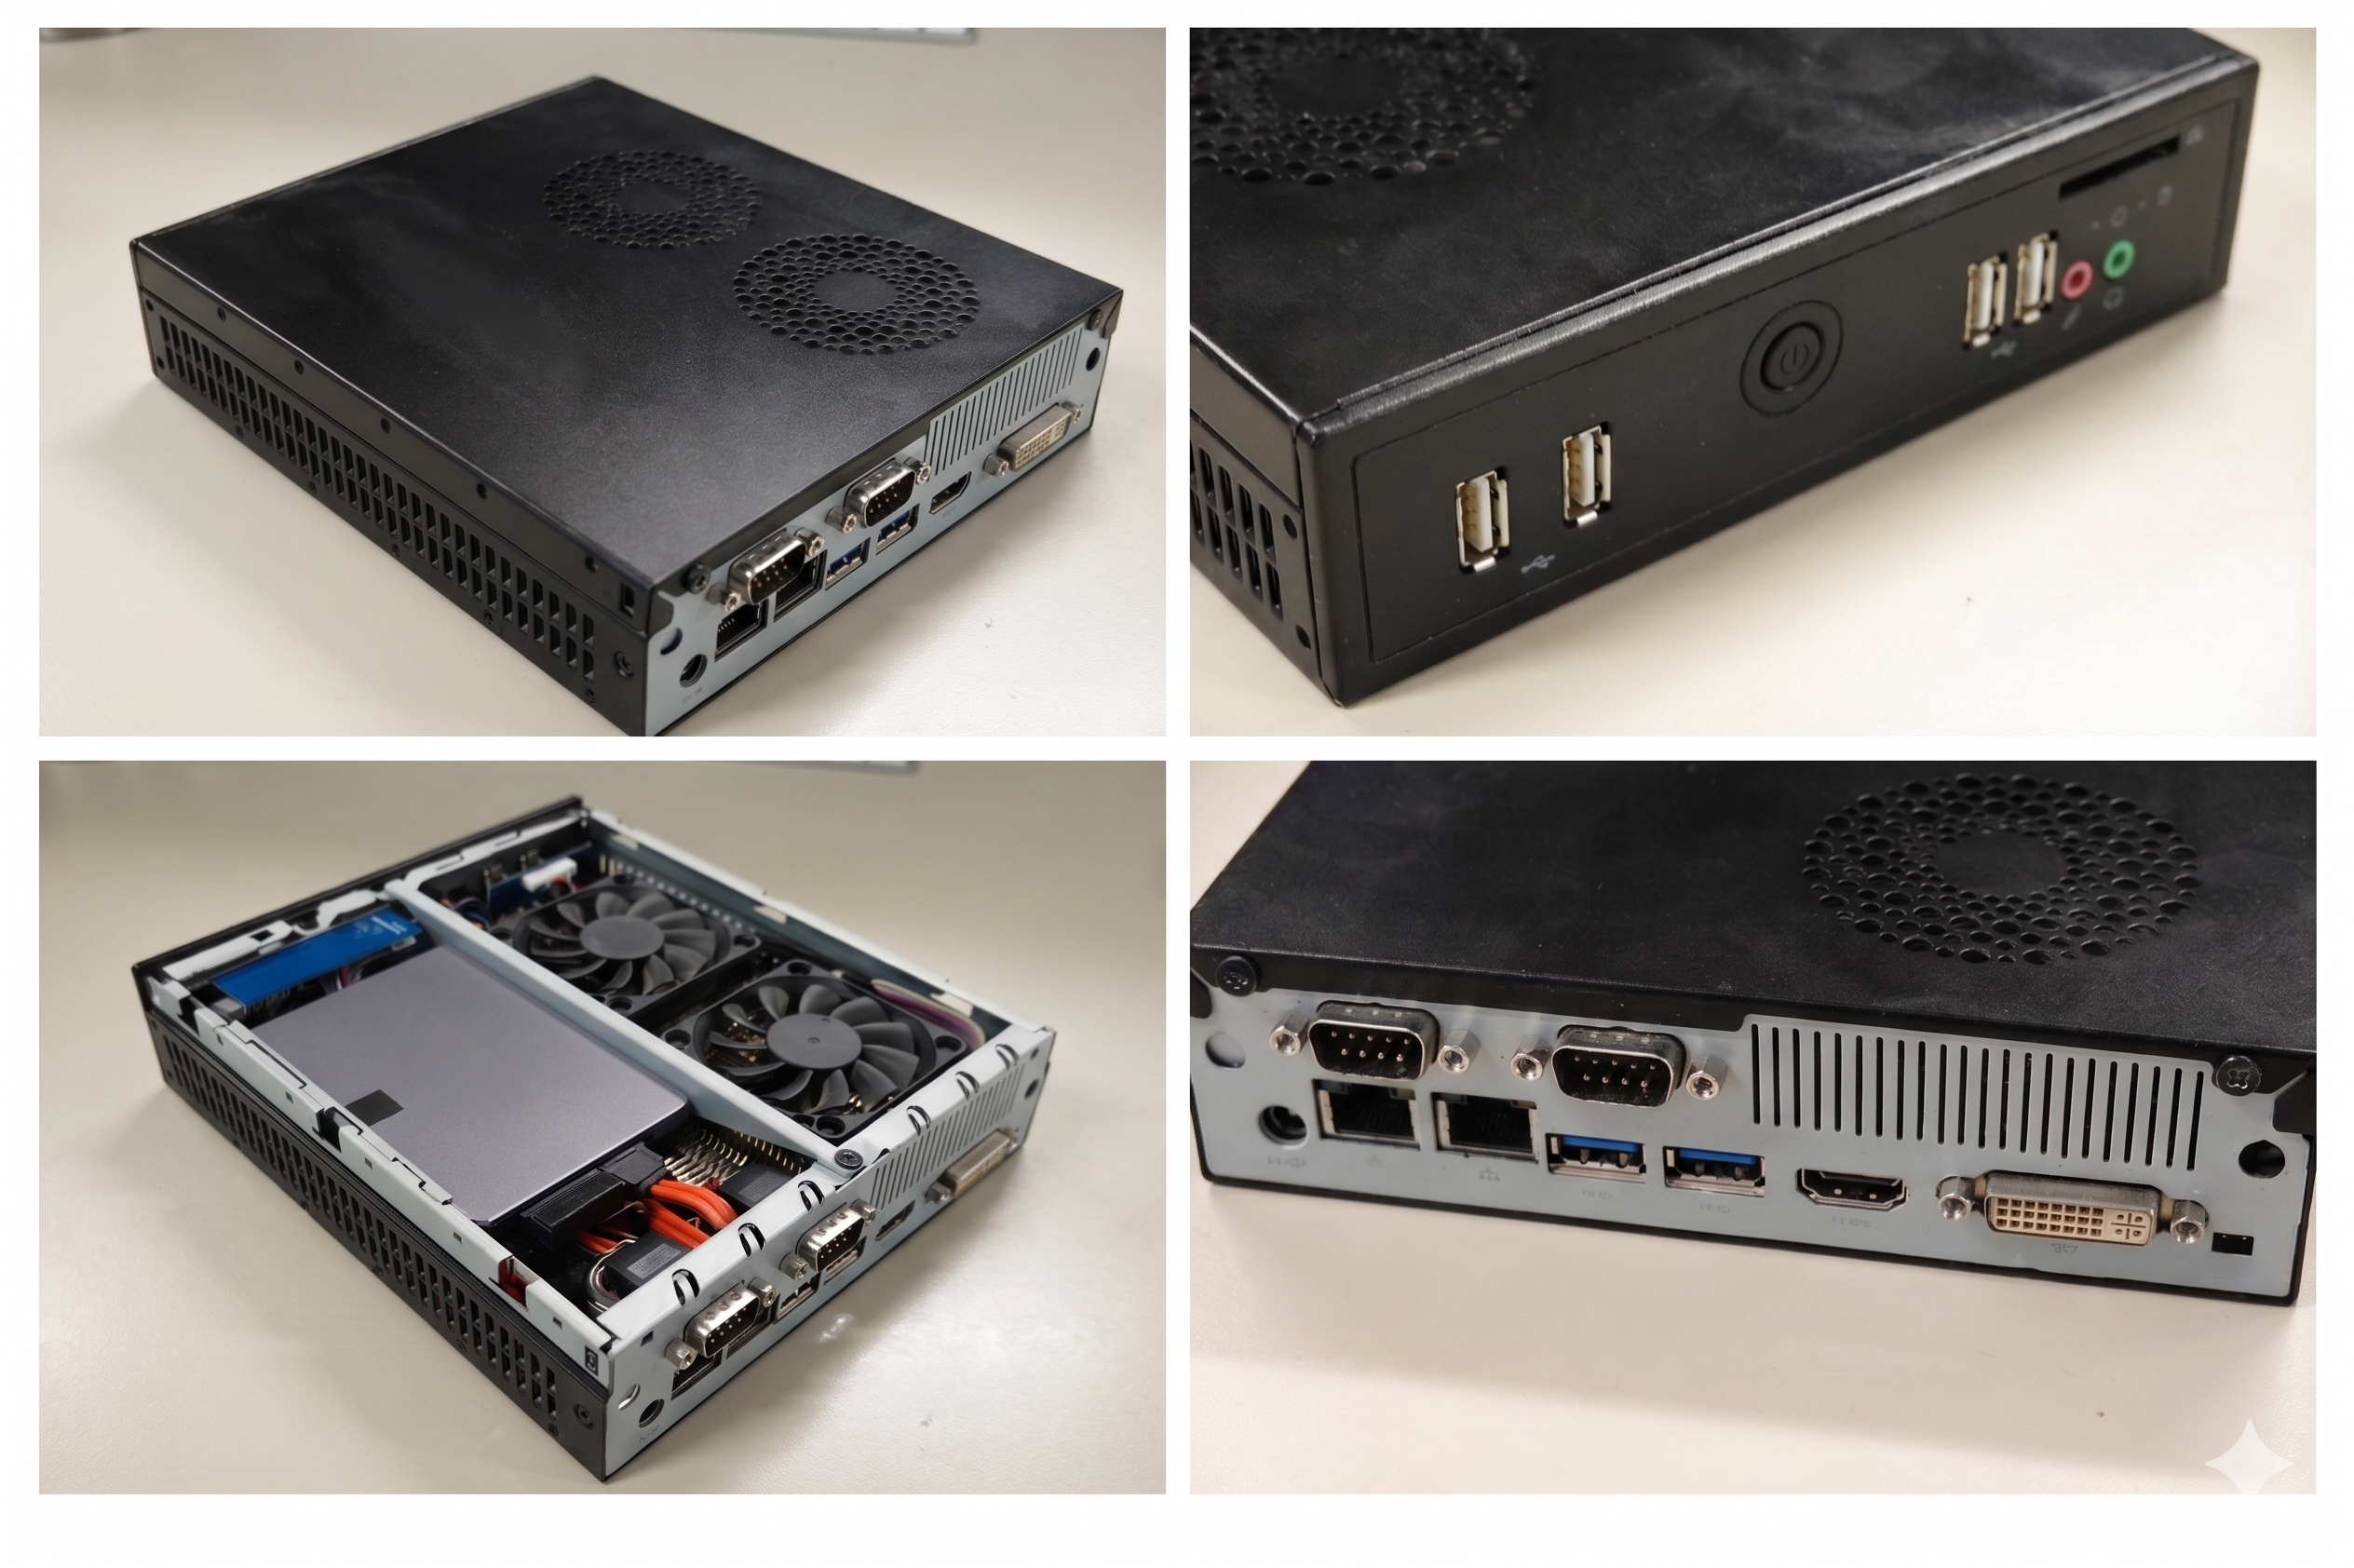
\includegraphics[width=0.9\linewidth]{include/foto.png}
\end{figure}

\begin{figure}[H]
	\centering
	\caption{UEFI - Einstellung}
	\label{fig:uefi}
	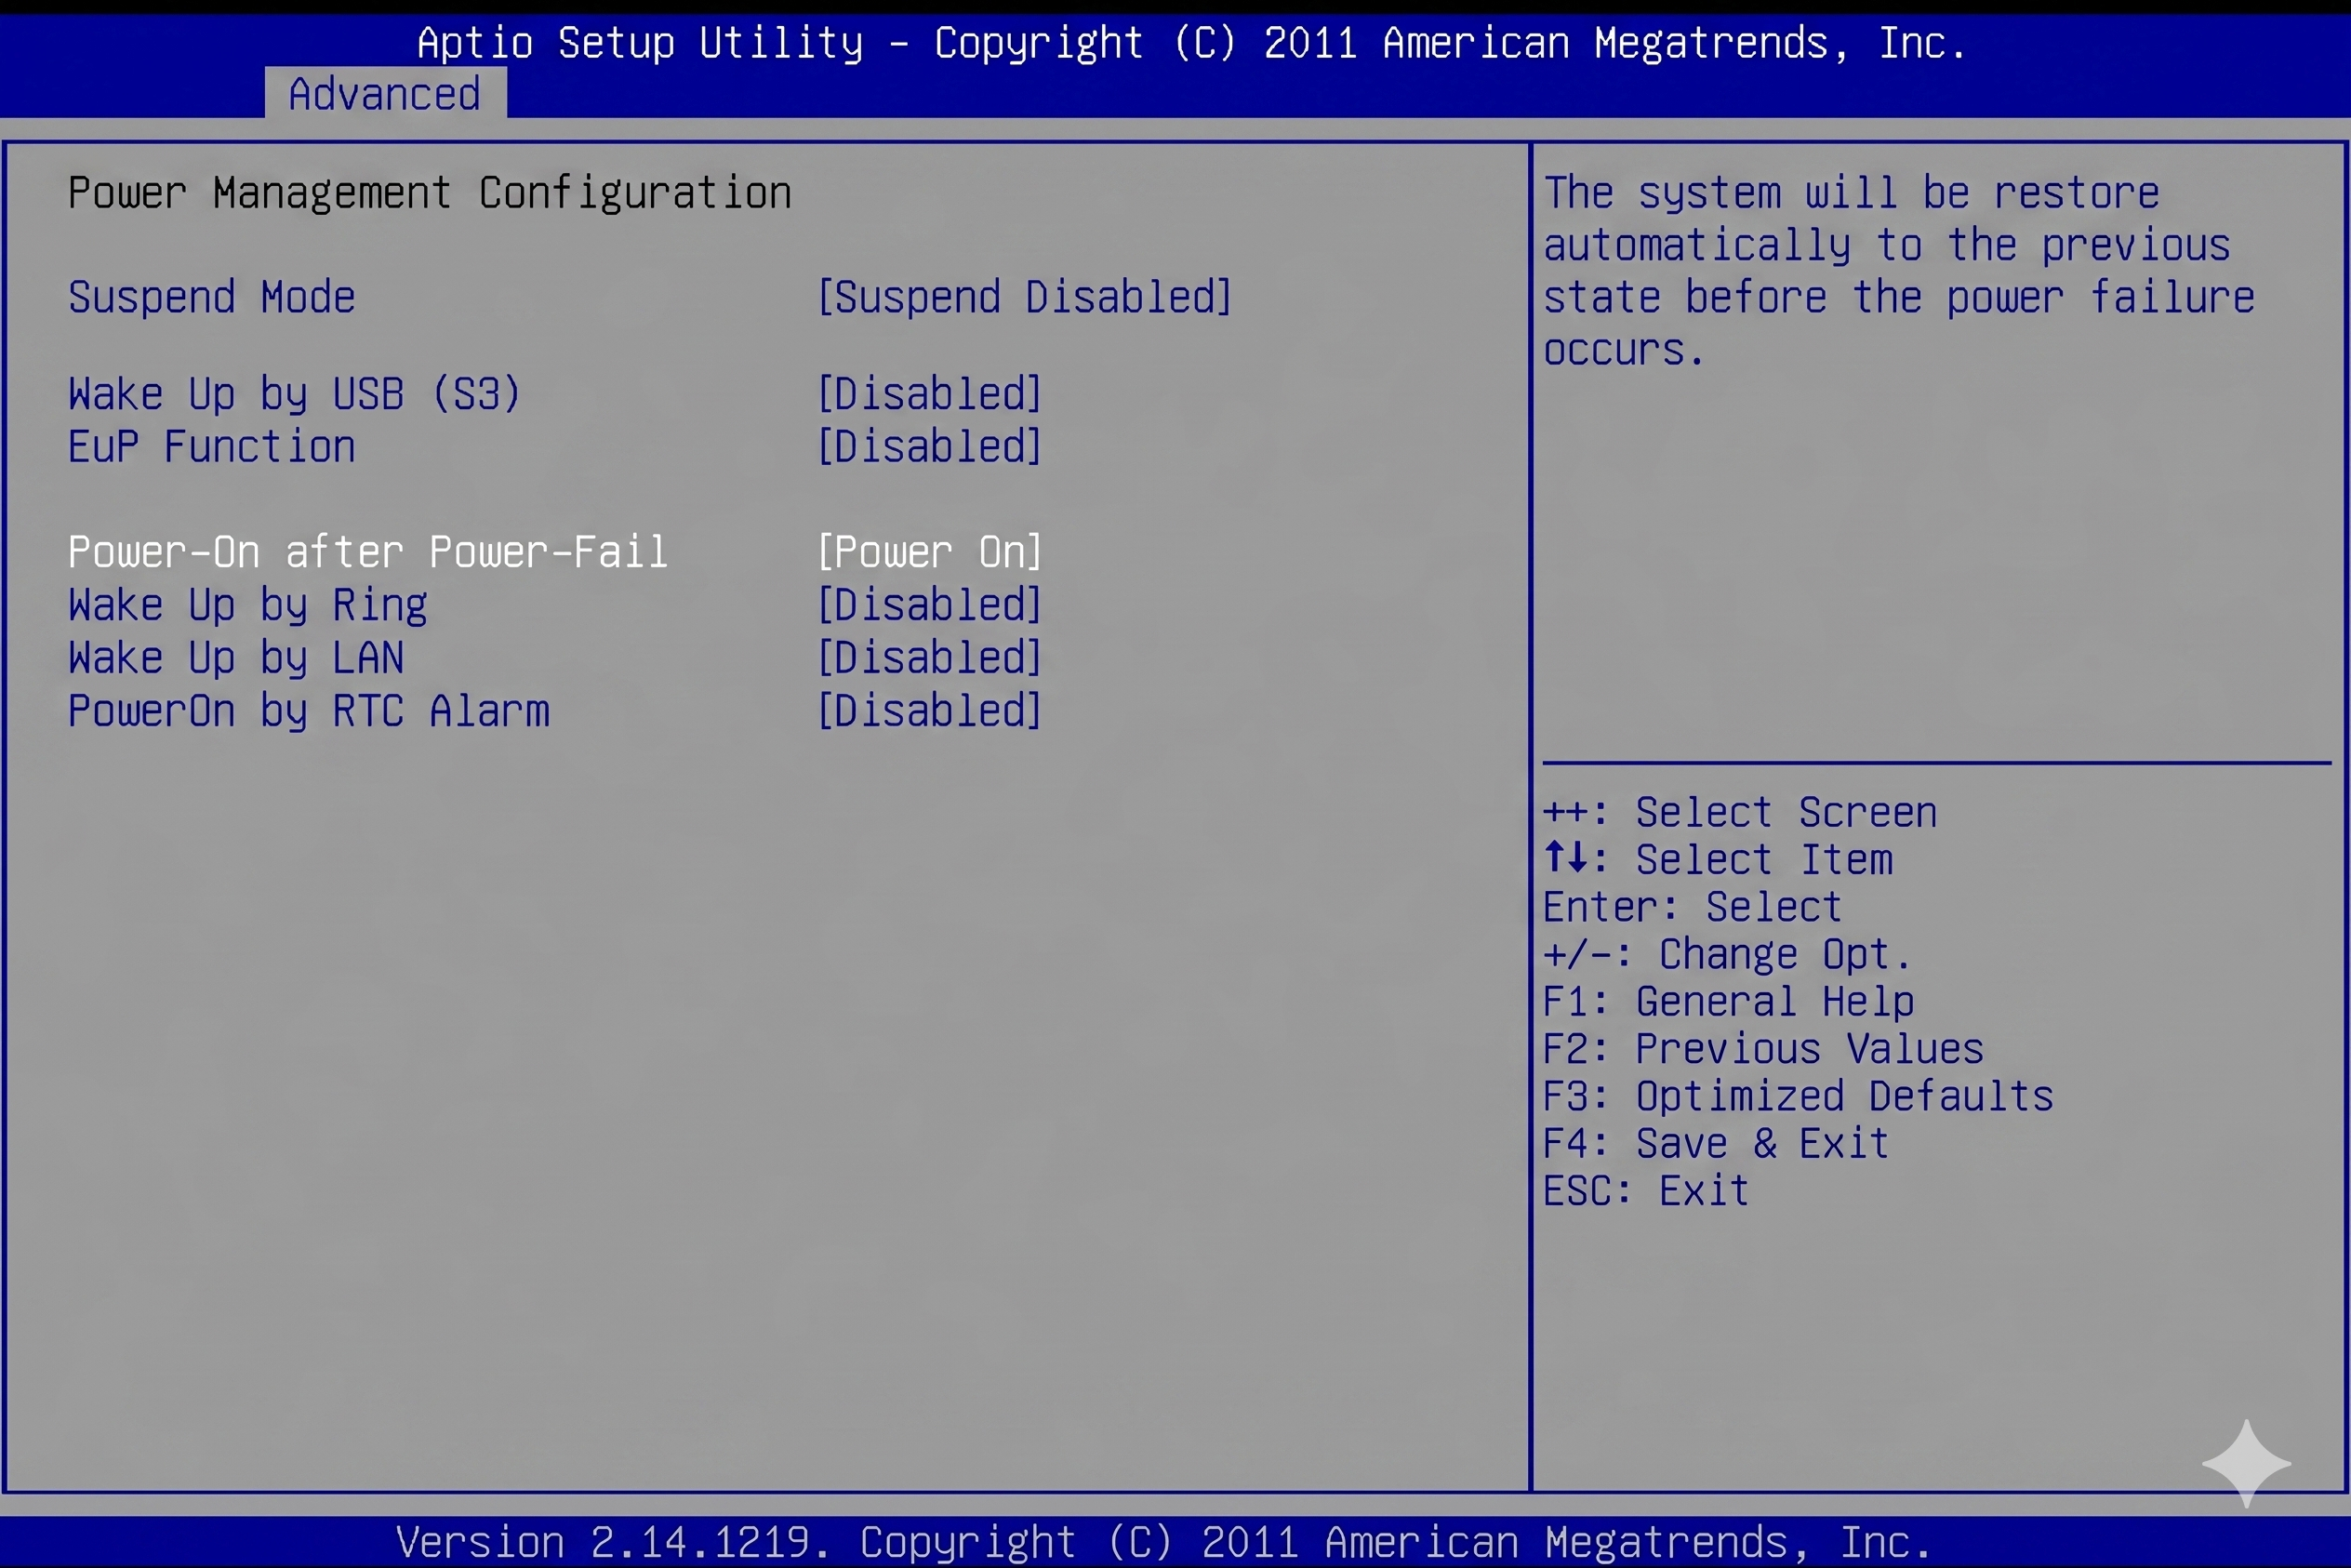
\includegraphics[width=0.9\linewidth]{include/UEFI.png}
\end{figure}

\begin{figure}[H]
	\centering
	\caption{LXD - Login}
	\label{fig:lxd}
	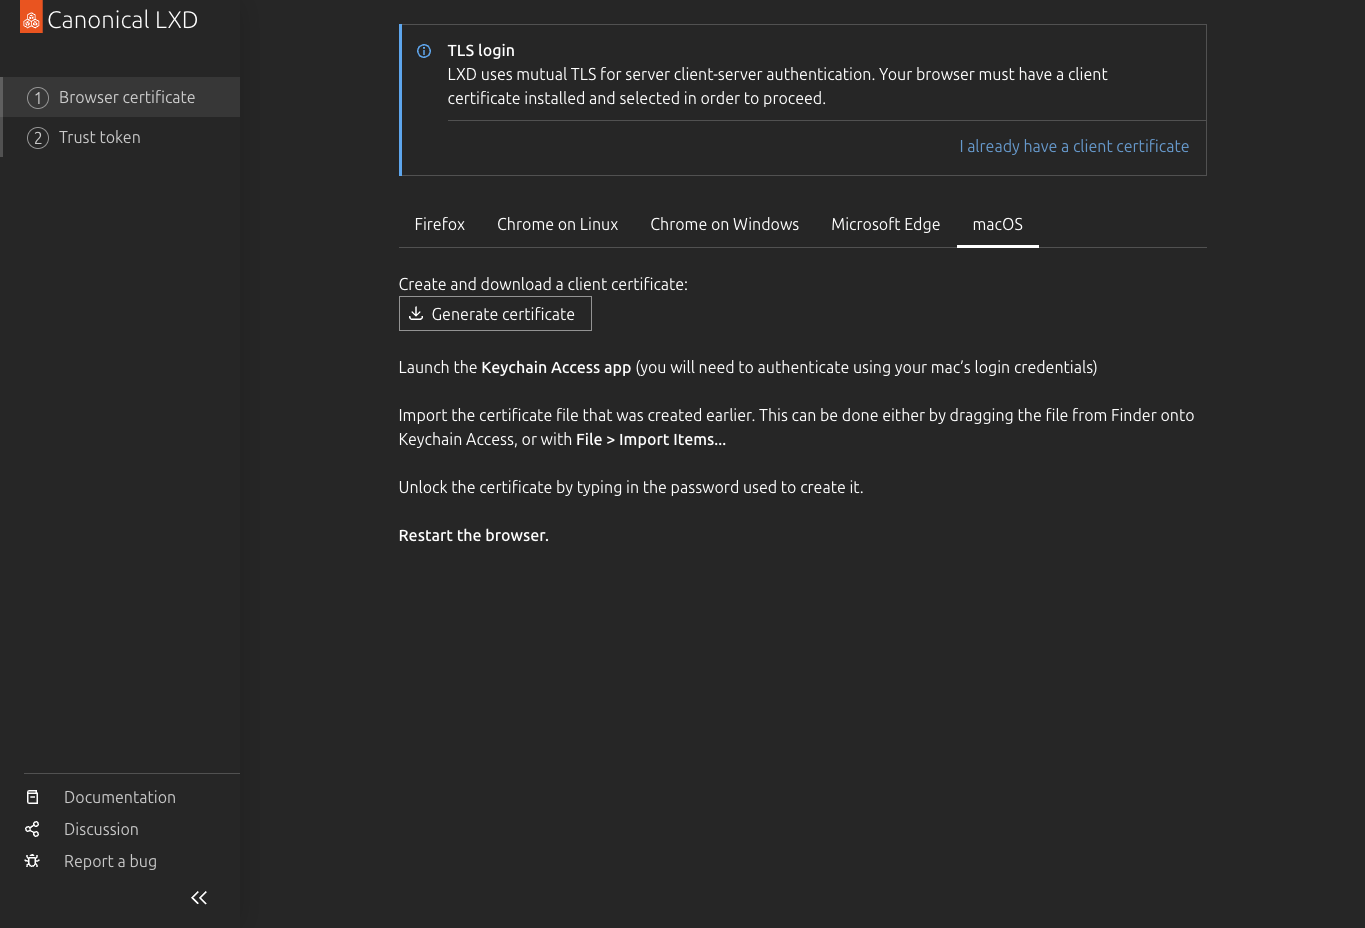
\includegraphics[width=0.9\linewidth]{include/LXD-Login.png}
\end{figure}

\begin{figure}[H]
	\centering
	\caption{Infrastructure - Hub}
	\label{fig:hub}
	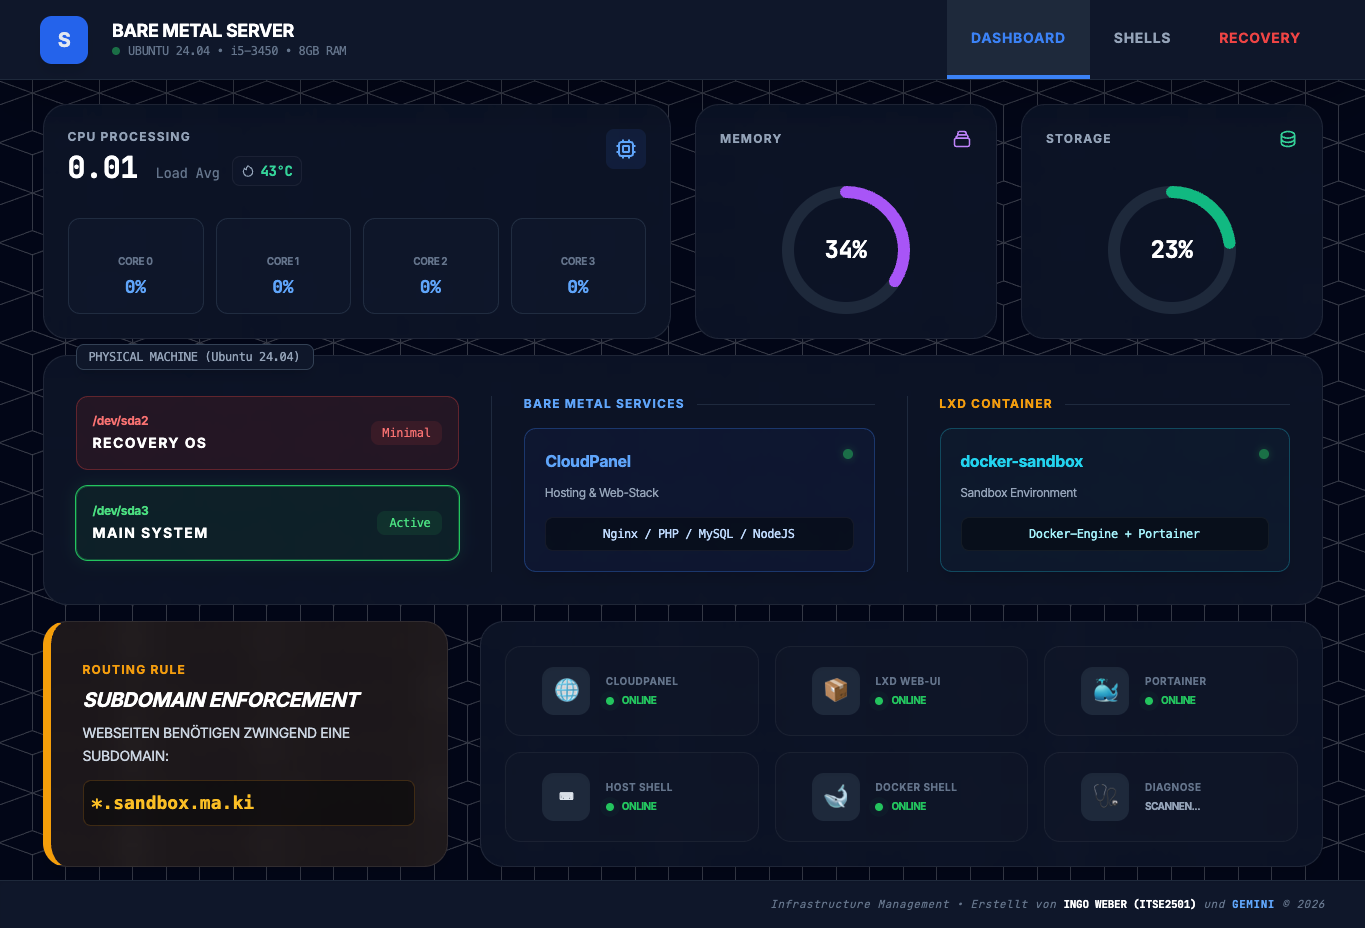
\includegraphics[width=0.9\linewidth]{include/hub.png}
\end{figure}

\begin{figure}[H]
	\centering
	\caption{Cloudpanel | Sites }
	\label{fig:cloudpanel}
	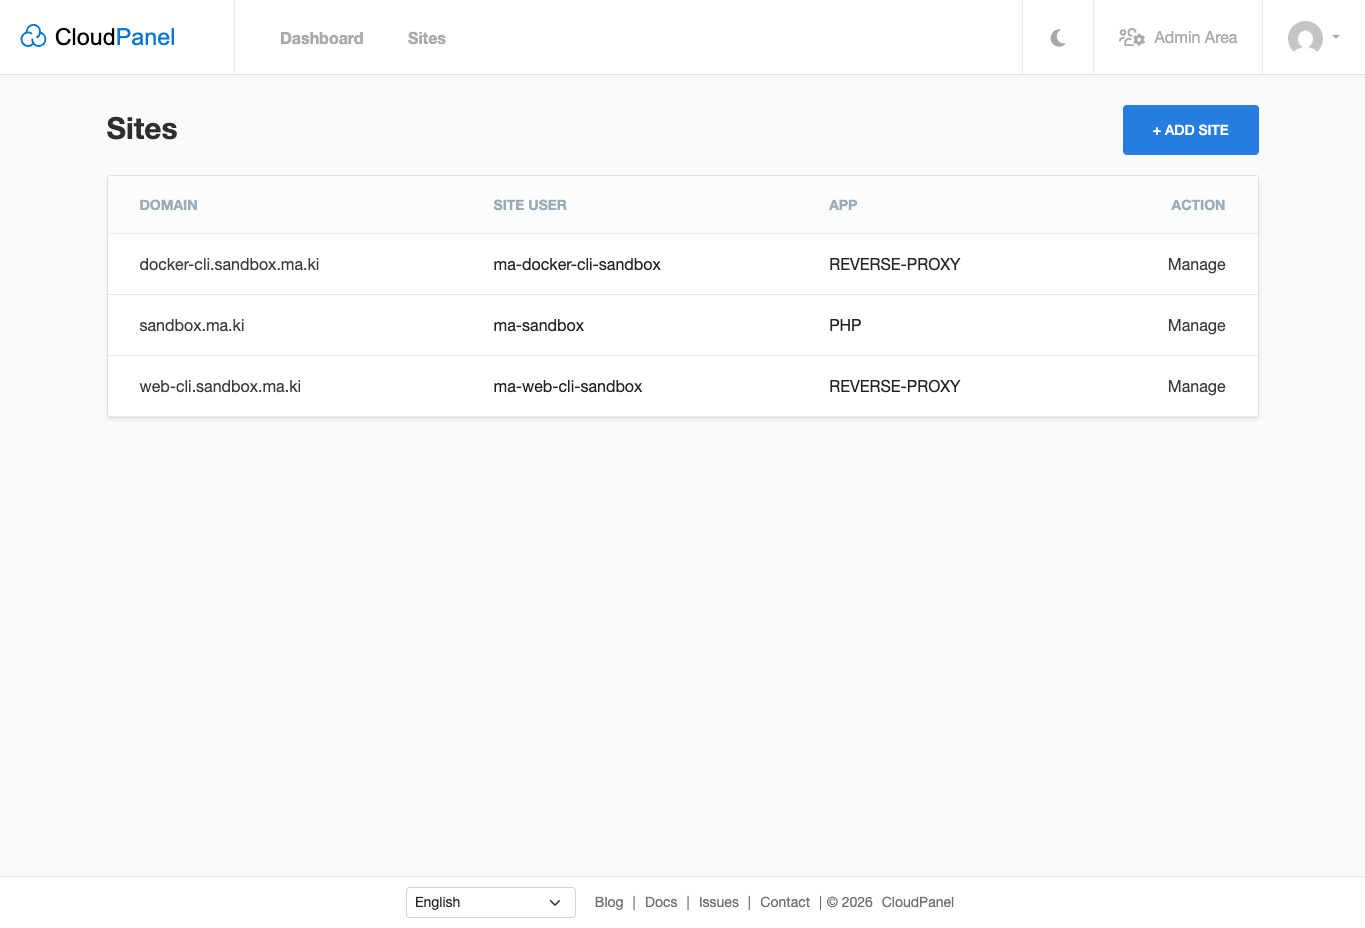
\includegraphics[width=0.9\linewidth]{include/cloudpanel.png}
\end{figure}

\begin{figure}[H]
	\centering
	\caption{Portainer | local}
	\label{fig:portainer}
	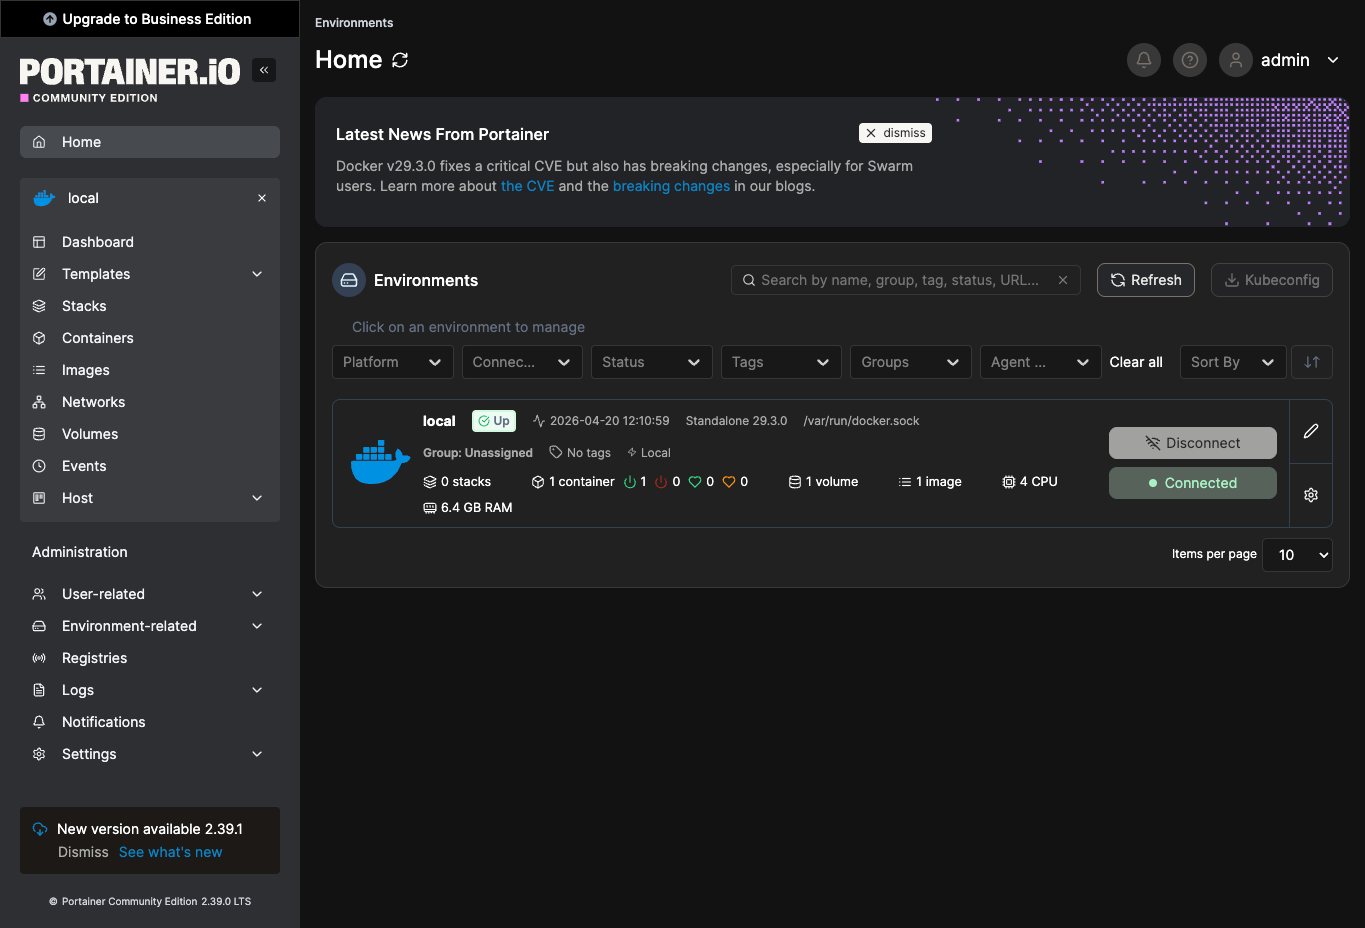
\includegraphics[width=0.9\linewidth]{include/portainer.png}
\end{figure}
\newpage
\section{Anlagen - Quelltexte}
\label{sec:quellcode}

\subsection{Beispiel-Custom Grub-Konfiguration  (40\_custom)} \label{sda3:grub}
\lstinputlisting[language=bash]{include/40_custom.grub.txt}
\bigskip

\subsection{Konfiguration von ttyd des Hauptsystems} \label{sda3:ttyd-web}
\lstinputlisting[language=bash]{include/ttyd-web.txt}
\bigskip

\subsection{Cronjob des Root-Nutzers} \label{sda3:cron}
\lstinputlisting{include/cronjob.txt}
\bigskip
\newpage
\subsection{Auto-Healer-Script (nginx-autohealer)} \label{sda3:healer}
\lstinputlisting[language=bash]{include/nginx-autohealer.sh}
\bigskip
\newpage
\subsection{Service-Script für den Factory-Reset (factory-reset.service)} \label{sda2:service}
\lstinputlisting{include/sda2-factory-reset.service}
\bigskip

\subsection{Shell-Script für den Factory-Reset (factory-restore.sh)} \label{sda2:shell}
\lstinputlisting[language=bash]{include/sda2-factory-restore.sh}
\bigskip

\subsection{Standard-Konfiguration der LXC-Container (default-profil.yaml)} \label{default-profil-yaml}
\lstinputlisting[language=XML]{include/default-profil.yaml} % YAML wird oft als XML/Ruby erkannt, oder 'bash' nutzen
\bigskip

\subsection{Konfigurationsdatei der Netzwerkschnittstelle MACVLAN (networks-macvlan0.yaml)} \label{macvlan-yaml}
\lstinputlisting[language=XML]{include/networks-macvlan0.yaml} % YAML wird oft als XML/Ruby erkannt, oder 'bash' nutzen
\bigskip

\subsection{Konfigurationsdatei der Netzwerkbrücke (networks-lxdbr0.yaml)} \label{netbr-yaml}
\lstinputlisting[language=XML]{include/networks-lxdbr0.yaml} % YAML wird oft als XML/Ruby erkannt, oder 'bash' nutzen
\bigskip

\subsection{Konfigurationsdatei des Docker-Containers (docker-sandbox.yaml)} \label{docker-yaml}
\lstinputlisting[language=XML]{include/docker-sandbox.yaml} % YAML wird oft als XML/Ruby erkannt, oder 'bash' nutzen
\bigskip
\newpage
\subsection{Konfiguration von ttyd des LXC-Containers} \label{sda3:ttyd-docker}
\lstinputlisting[language=bash]{include/ttyd-docker.txt}
\bigskip

\subsection{Ausschnitt der PHP-Datei des Dashboards (index.php)} \label{app:php_code}
\lstinputlisting[language=PHP]{include/index_a.php}
\bigskip

\subsection{Ausschnitt der Design-Anpassungen (style.css)} \label{app:css_style}
\lstinputlisting[language=HTML]{include/style_a.css}
\bigskip

\subsection{vHost des Reverse-Proxies Hauptsystem-TTYd} \label{vhost:web}
\lstinputlisting[language=bash]{include/web-cli.sandbox.vhost.txt}
\bigskip

\subsection{vHost des Reverse-Proxies Container-TTYd} \label{vhost:docker}
\lstinputlisting[language=bash]{include/docker-cli.sandbox.vhost.txt}

\newpage
\section{Anlagen - Hostnamen, IP-Adressen, Initial-Passwörter} \label{sec:pass}

\begin{table}[H]
	\centering
	\caption{Detaillierte Dienst- und Portmatrix der Sandbox}
	\begin{tabular}{llll}
		\hline
		\textbf{Dienst} & \textbf{IP-Adresse} & \textbf{Port} & \textbf{URL} \\ \hline
		Web-Server (Hub)   & \texttt{192.168.100.21} & 443   & \texttt{https://sandbox.ma.ki/} \\
		CloudPanel UI      & \texttt{192.168.100.21} & 8443  & \texttt{https://sandbox.ma.ki:8443/} \\
		LXD Dashboard      & \texttt{192.168.100.21} & 9443  & \texttt{https://sandbox.ma.ki:9443/} \\
		SSH-Host (Hauptsystem)          & \texttt{192.168.100.21} & 22    & \texttt{ssh://web@sandbox.ma.ki} \\
		Portainer UI    & \texttt{192.168.100.22} & 9443   & \texttt{https://docker-sandbox.ma.ki:9443/} \\ \hline
	\end{tabular}
\end{table}

\begin{table}[H]
	\centering
	\caption{Initial-Passwörter}
	\begin{tabular}{lll}
		\hline
		\textbf{Dienst} & \textbf{Username} & \textbf{Passwort} \\ \hline
		Recovery Shell/SSH   & agent & IT123\_maki \\
		Hauptsystem Shell/SSH      & web & IT123\_maki \\
		Cloudpanel UI & admin         & IT123\_maki \\
		Docker LXC Shell         & root & IT123\_maki \\
		Portainer UI          & admin & IT123456\_maki \\ \hline
	\end{tabular}
\end{table}

\newpage
\vspace*{\fill}
\section{Anlagen - Kundendokumentation}\label{sec:kd}
\vspace*{\fill}

\includepdf[pages=-, frame=true, scale=1]{Kundendokumentation.pdf}

\newpage
\DeclareFieldFormat{url}{\newline\url{#1}}
\DeclareFieldFormat{urldate}{\newline(abgerufen am #1)}
\nocite{*} % Nimmt alle Quellen aus der .bib-Datei auf, auch ohne \cite
% An der Stelle, an der das Verzeichnis gedruckt werden soll:
\printbibliography[title={Quellenverzeichnis}, heading=bibintoc]
\label{sec:quellen}

\end{document}  %beendet das Dokument